% ================================================================

\documentclass[a4paper]{article}

% ------------------------- Project metadata
% \usepackage{sansmath}
\newcommand{\ProjectTitle}{$\boldsymbol{\beta}$-boost}
% \newcommand{\ProjectTitle}{$\sansmath{\mathsf{\beta}}$-boost}
\newcommand{\ProjectSubTitle}{Simulating Special Relativity in Unity}
\newcommand{\ProjectDescription}{Final project report}
\newcommand{\CourseName}{Models and Simulation}
\newcommand{\CourseCode}{DD1354}

% ------------------------- Preamble
\usepackage{KTHpreamble}        % Custom preamble
\addbibresource{refs.bib}       % References


\author{%
  \begin{flushleft}
  \textbf{Axel Hammarskiöld Spendrup}\\
  Email: \textit{\href{mailto:axelhs@kth.se}{axelhs@kth.se}}\\[1ex]
  Source code: \textit{\href{https://github.com/4xwell/beta-boost}{Github repository}}\\
  Project blog: \textit{\href{https://lorentztransform.wordpress.com}{lorentztransform.wordpress.com}}\\[1ex]
  {Grade aim: \textbf{A}}
  \end{flushleft}
}

\date{%
  \begin{flushleft}
  Stockholm, Sweden\\
  \today
  \vspace*{-5em}
  \end{flushleft}
}

% ================================================================

\begin{document}

% ------------------------- Title page
\maketitle
\thispagestyle{titlepage}

\begin{tikzpicture}[remember picture, overlay]
    \node[anchor=north east, inner sep=72pt, yshift=-18pt] at (current page.north east) 
    {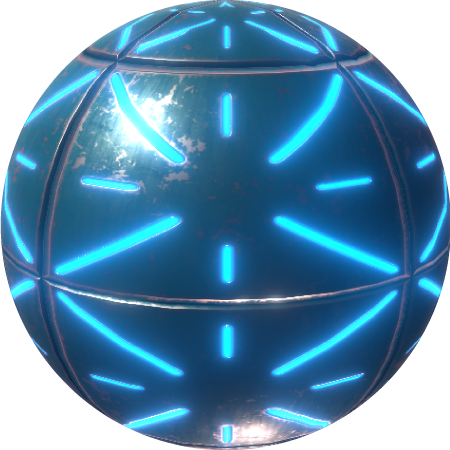
\includegraphics[width=3cm]{img/ball.png}};
    % {\includesvg[width=3cm]{KTH_logo_RGB_bla.svg}};
\end{tikzpicture}


% ------------------------- Abstract
\section*{Abstract}
This project seeks to bridge the gap between theoretical knowledge and physical intuition of relativistic effects, in particular the length contraction phenomenon. It implements a three-dimensional, virtual simulation built in the Unity game engine, allowing users to interactively explore the physics of special relativity in real-time. Inspired by the concept of natural units, the speed of light in the simulation is artificially reduced, thereby visualizing relativistic effects at velocities more familiar to everyday life. The simulation calculates velocity based parameters, $\beta$ and $\gamma$, to construct a Lorentz transformation matrix at each time step. The matrix is then applied to the vertices of static environment meshes via CPU computations at runtime. The resulting visualization illustrates the connection between the 4-vector formalism of Minkowski spacetime and the observable geometric distortions of the environment as predicted by special relativity, in particular length contraction.

% This project seeks to address the conceptual and educational challenges of comprehending Special Relativity, particularly the phenomenon of relativistic length contraction. Using Unity’s real-time 3D engine, we implement a per-vertex Lorentz transformation on objects, allowing users to interactively experience and visualize how lengths contract as relative velocity increases. The system calculates velocity-based parameters in a dedicated player controller script and applies a corresponding Lorentz boost matrix to every vertex of the scene geometry at runtime. In doing so, it illustrates the direct link between relativistic equations and observable geometric effects. The methodology emphasizes clarity and correctness: it avoids shader-based manipulations to maintain debuggable, educationally transparent code. Results confirm that measured contraction factors match theoretical predictions $L' = L/\gamma$. The project thereby offers a robust pedagogical tool that merges rigorous physics and interactive visualization, showcasing how game engines can serve as powerful platforms for science education.

% This report presents the design and implementation of a Unity-based simulation tool that illustrates key phenomena of Special Relativity, focusing on Lorentz transformations and length contraction. By leveraging real-time mesh manipulation, each vertex in the scene is re-positioned according to a 4D Minkowski boost matrix, enabling users to observe how objects aligned with the velocity appear contracted. We begin with foundational relativistic equations, then detail two development approaches---an earlier anisotropic scaling method and a final per-vertex transformation method. Our results demonstrate visually realistic contraction effects consistent with theoretical expectations, all within a standard game engine workflow. This project aims to serve as an educational platform, facilitating better intuition of relativistic concepts through interactive 3D visualization.


\clearpage


% ------------------------- Table of Contents
{\NoRule
\titlespacing{\section}{0em}{2em}{-2em}
\tableofcontents
\addtocontents{toc}{~\hfill \textsf{\footnotesize{Page}}\vspace{1em}\par}}
\clearpage


% ------------------------- Introduction
\NoRule
\section{Introduction}
An observer traveling at velocities close to the speed of light will experience exotic phenomena that constitute a unique and unintuitive part of physics. At these extreme velocities, the fabric of spacetime appears distorted from the observer's perspective, causing them to perceive, among other things, how distances become shorter and time intervals appear longer compared to measurements made in a rest frame.

The effects were initially predicted by Albert Einstein who modeled the behavior in his third \textit{annus mirabilis}\cite{annus} paper \textit{On the Electrodynamics of Moving Bodies} (1905)\cite{einstein}, later known as the \textit{special theory of relativity}. The theory rewrote the laws imposed by Newtonian mechanics for high velocities and revolutionized our perception of space and time.

While the effects of special relativity are present for every object in the universe at all velocities, they are only pronounced at extremely high speeds relative to the speed of light, $c$. Moreover, they are modeled mathematically as Lorentz transformations within Minkowski spacetime, an inherently abstract modification of a 4-dimensional manifold. This renders the effects virtually imperceptible in everyday life, posing an educational challenge for students accustomed to our relatively slow, 3-dimensional reality. The mathematical abstraction can leave a gap between theoretical knowledge and intuitive understanding.

This project addresses this gap through a real-time, interactive simulation, implemented in the 3D game engine Unity. The aim is to visually demonstrate the geometric consequences of Lorentz transformations, primarily length contraction, by artificially reducing the speed of light. This provides students and users with an intuitive feel for how these transformations manifest visually as relativistic effects. The initial project specification, outlining the goals and preliminary plan, can be found in Appendix \ref{appendix:specification}.

\renewcommand{\SectionRule}{\titlerule[.5pt]}

% }

%This project aims to allow anyone to experience the effects of special relativity, well below the extreme velocities required in reality. By constructing a special relativity simulation within the context of a computer game, the player of the game will get a better intuition of some notable relativistic effects such as length contraction, Lorentz boosts, coordinate transformations and more.

%The game will be built as an interactive 3D environment using Unity. The simulation scripts will be built on the rigorous mathematics of Lorentz transformations in Minkowski space that underpins special relativistic theory. By using natural units, (normalizing the speed of light to 1: c = 1 ), the relativistic effects will be prominent at velocities more familiar to us.


% -------------------------------------------------------------
% Background and theory

\section{Background}

Below is a theoretical background on the underpinnings of the special theory of relativity. It provides the fundamental mathematical framework required to understand the simulation, together with examples of how relativistic effects manifest.

The mathematical formalism employed in this project is primarily derived from Wolfgang Rindler's \textit{Introduction to Special Relativity} \cite{rindler}. All mathematical derivations in this report follow from this book, except where explicitly indicated otherwise. 

\subsection{Postulates of special relativity}

Special relativity is built on two fundamental postulates:

\begin{postulate}[Principle of Relativity]
    The laws of physics take the same form in all inertial frames of reference.
\end{postulate}

\begin{postulate}[Invariance of the Speed of Light]
    As measured in any inertial frame of reference, light is always propagated in empty space with a definite velocity c that is independent of the state of motion of the emitting body. Or: the speed of light in free space has the same value c in all inertial frames of reference.
\end{postulate}

\noindent
The mathematical structure of special relativity, particularly the Lorentz transformations, follows logically from these two postulates, along with additional assumptions such as the homogeneity and isotropy of space and time \cite{postulates}.


% \subsection{Mathematical formalism}
\subsection{Minkowski spacetime}
The calculations of special relativity pertinent to the simulation concern linear transformations between different inertial frames of reference. In these inertial frames, often denoted as \(S \text{ and } S'\), each instance in space and time is a unique point known an \textit{event}, represented as a four-dimensional vector (4-vector): $X = (ct,\  x,\ y,\ z)$. These vectors exist on a 4-dimensional flat manifold known as \textit{Minkowski space}, constructed from three spatial dimensions plus time.

When comparing events between different inertial frames, one frame $S$ is often designated as the \textit{rest frame} relative to the objects being observed, while the other frame $S'$ moves with constant velocity relative to $S$. It is possible to define a spacetime interval $\Delta s^2$ between two events, \(X_1 \text{ and } X_2\), which is invariant under transformations between inertial frames. Using the metric signature \((+,-,-,-)\), the interval is
\begin{equation}
    \Delta s^2 = (c\,\Delta t)^2 - \Delta x^2 - \Delta y^2 - \Delta z^2, \label{interval}
\end{equation}
where $\Delta t = t_2 - t_1,\ \Delta x = x_2 - x-1$ etc. The invariance of this interval is a direct consequence of the postulates.

\begin{figure}[ht]
    \centering
    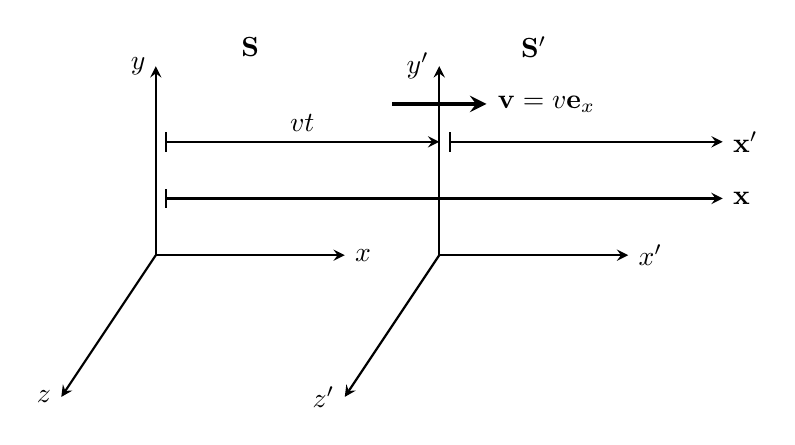
\begin{tikzpicture}[>=stealth, scale=1.2]
    
        % Axes for frame S
        \draw[->, thick] (0,0) -- (2,0) node[right] {$x$};
        \draw[->, thick] (0,0) -- (0,2) node[left] {$y$};
        \draw[->, thick] (0,0) -- (-1,-1.5) node[left] {$z$};
        
        % Axes for frame S'
        \draw[->, thick] (3,0) -- (5,0) node[right] {$x'$};
        \draw[->, thick] (3,0) -- (3,2) node[left] {$y'$};
        \draw[->, thick] (3,0) -- (2,-1.5) node[left] {$z'$};
        
        % Labels for frames
        \node at (1, 2.2) {$\mathbf{S}$};
        \node at (4, 2.2) {$\mathbf{S'}$};
        
        % Arrows indicating velocity and displacement
        \draw[|->, thick] (0.1, 1.2) -- (3, 1.2) node[midway, above] {$vt$};
        \draw[|->, thick] (0.1, 0.6) -- (6, 0.6) node[right] {$\mathbf{x}$};
        \draw[|->, thick] (3.1,1.2) -- (6, 1.2) node[right] {$\mathbf{x}'$};
        \draw[->, ultra thick] (2.5,1.6) -- (3.5, 1.6) node[right] {$\mathbf{v}=v\mathbf{e}_x$};
    
    \end{tikzpicture}
    \caption{Schematic representation of two inertial frames, \(S\) at rest and \(S'\) moving with constant velocity \(\vec{v}\) along the positive x-axis. The diagram illustrates relationships between coordinates.}
    \label{fig:two-frames}
\end{figure}

\subsection{Lorentz transformations}
The Lorentz transformation is the linear transformation relating the spacetime coordinates of an event as measured in two different inertial frames, \(S \text{ and } S'\), moving with constant velocity relative to each other. The transformation can include a spatial rotation and a velocity boost. If the relative motion involves no rotation, the transformation is referred to as a \textit{Lorentz boost}, illustrated schematically in figure \ref{fig:boost}. A key property of the transformation is \textit{Lorentz invariance}: it preserves the spacetime interval \eqref{interval} between any two events when calculated in either frame.

\begin{figure}[ht]
    \centering
    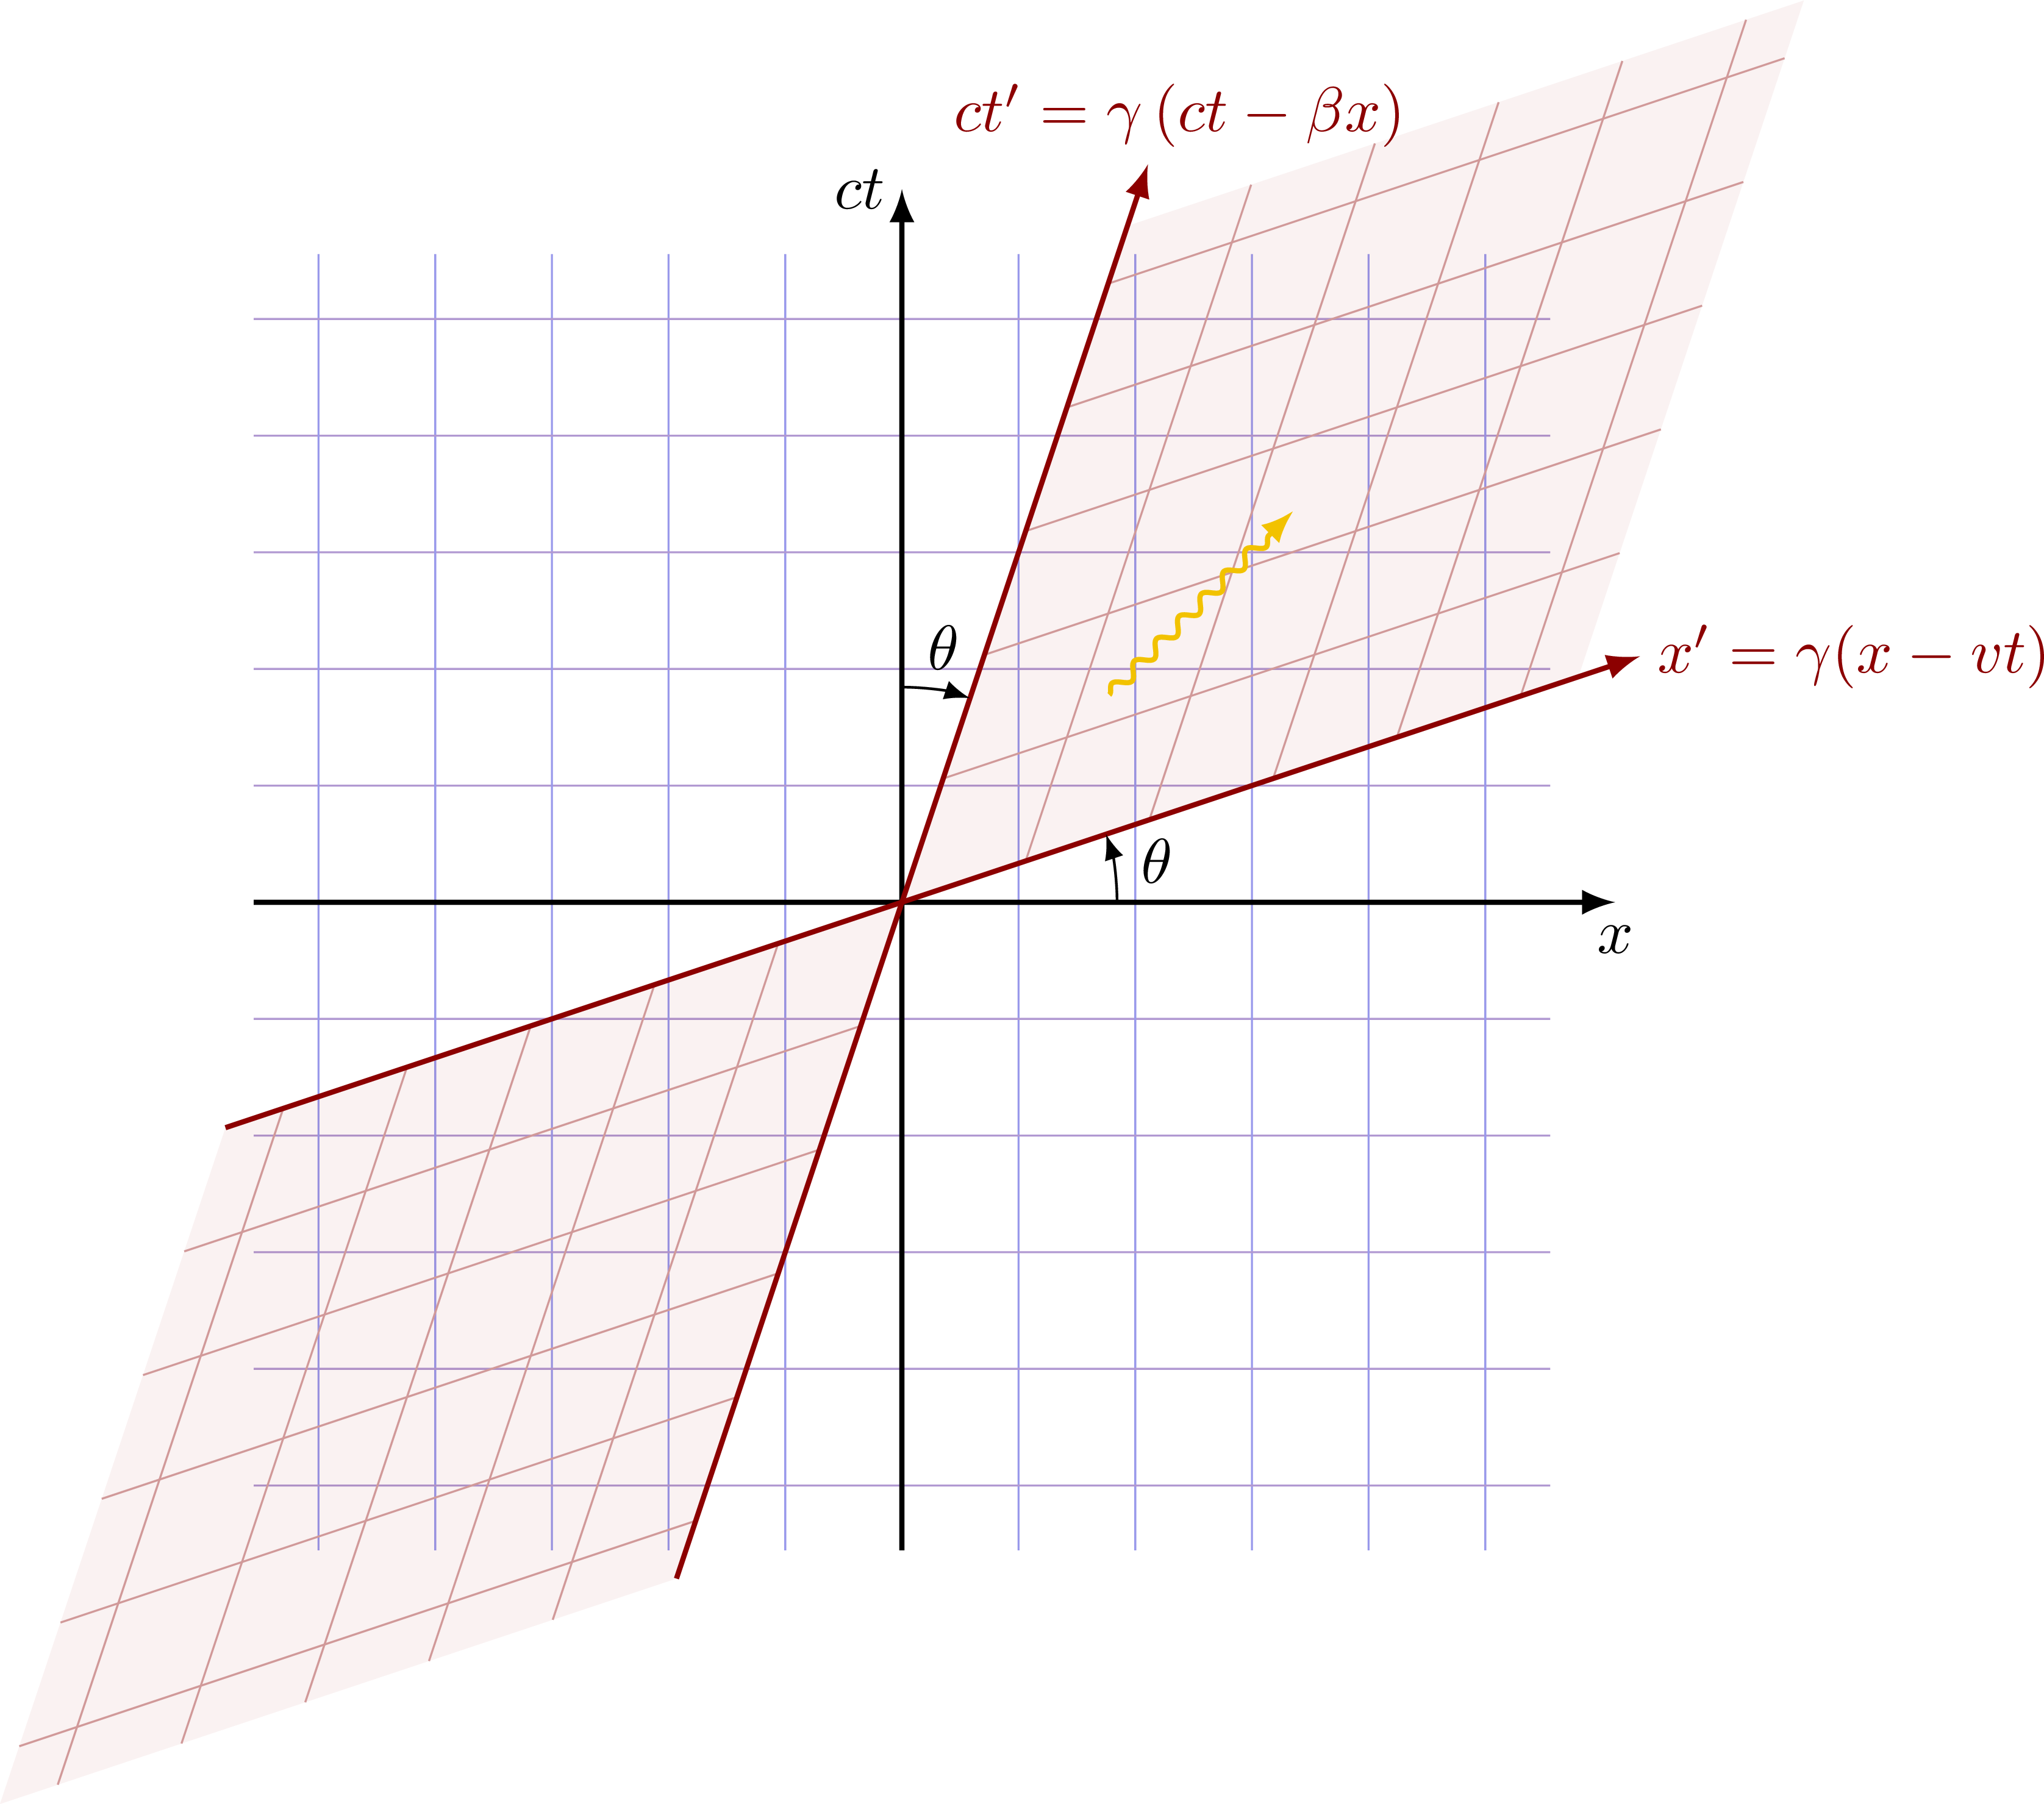
\includegraphics[width=0.49\linewidth]{img/lorentz boost.png}
    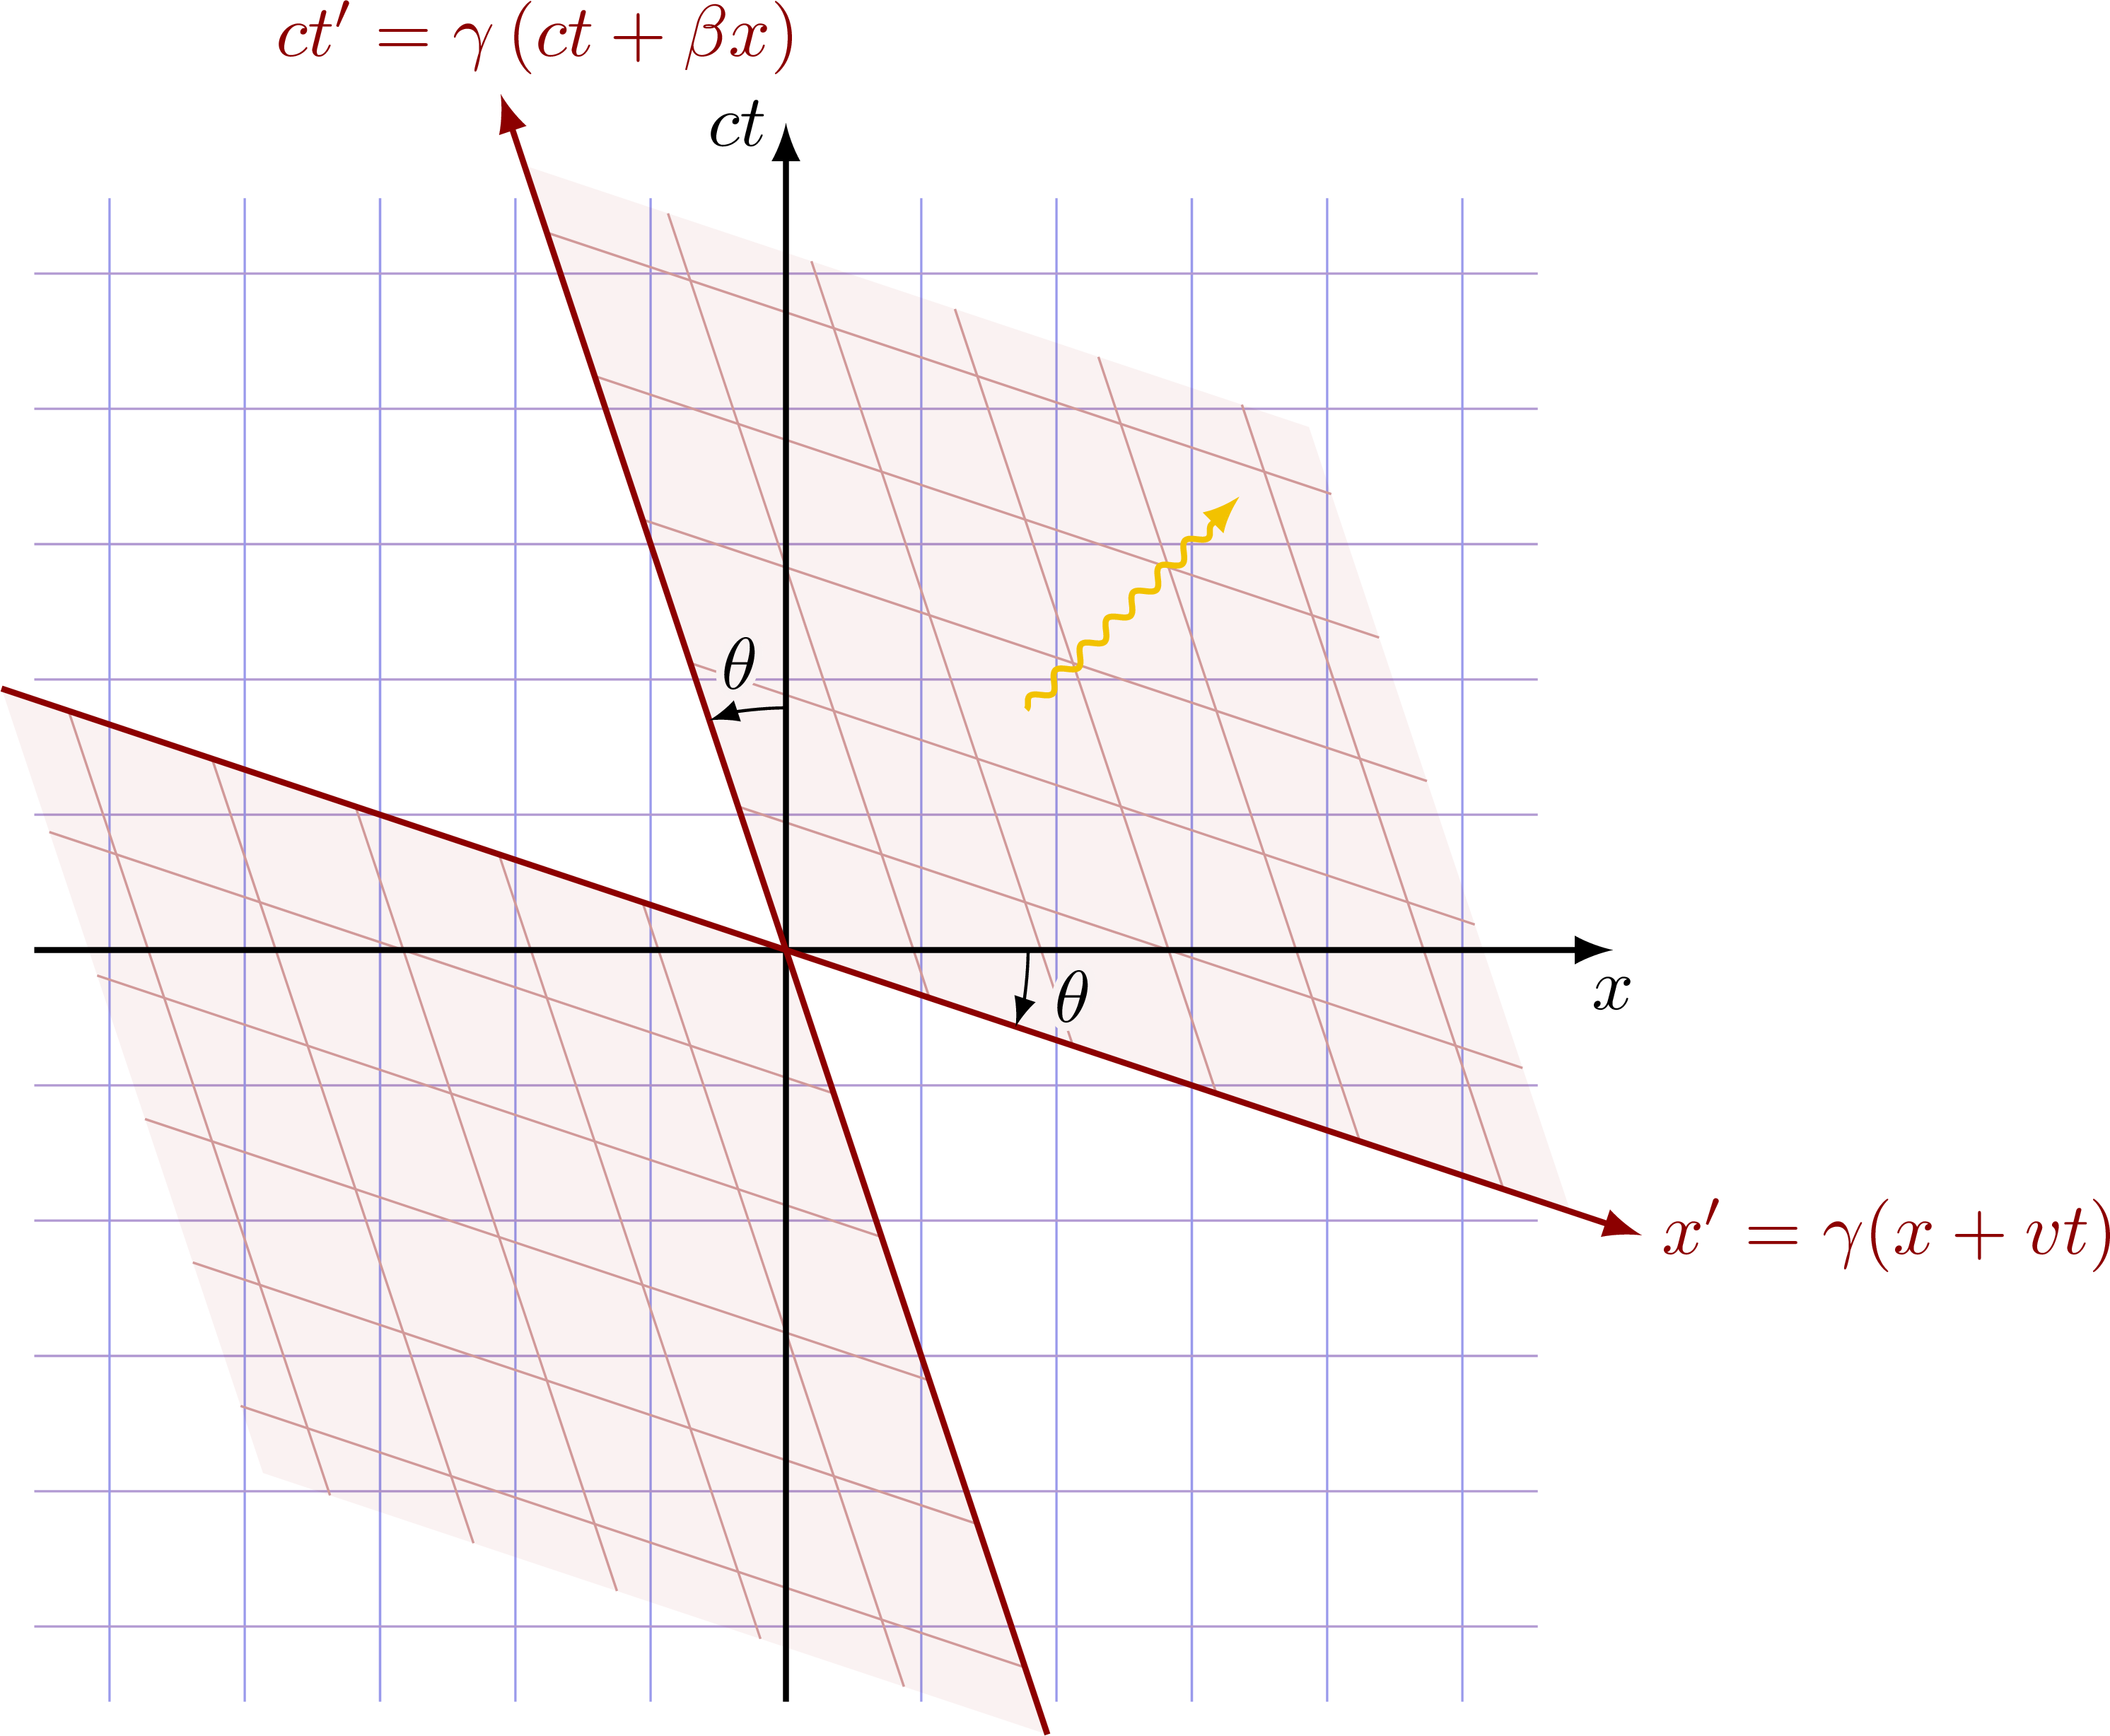
\includegraphics[width=0.49\linewidth]{img/inverse boost.png}
    \caption{\textbf{Left:} Spacetime diagram illustrating a Lorentz boost for a frame $S'$ moving in the positive x-direction relative to $S$. Note that the $x'$ and $ct'$ axes are tilted at an equal angle $\theta$ relative to the $x$ and $ct'$ axes. \textbf{Right:} The inverse transformation, equivalent to observing $S$ from $S'$, where $S$ moves in the negative x-direction relative to $S'$. The angle $\alpha$ is given by $\tanh \alpha = \beta = v/c$ \cite{tikz}.}
    %\caption{\textbf{Left:} Lorentz transformation of a boosted frame moving in the positive x-direction. \textbf{Right:} the inverse Lorentz transformation, equivalent to a boosted frame moving in the negative x-direction. The angle $\theta$ is given by the relation $\beta = \frac{v}{c} = \tan\theta$ \cite{tikz}.}
    \label{fig:boost}
\end{figure}

Mathematically, the transformation is represented as the matrix multiplication $X' = \Lambda X$, where $X$ and $X'$ are the 4-vector representations of the same event in frames $S$ and $S'$ respectively, and $\Lambda$ is the \textit{Lorentz transformation matrix}. For the specific case where $S'$ moves with velocity $\mathbf{v} = v\mathbf{e}_x$ relative to $S$ as in figure \ref{fig:two-frames}, the transformation is calculated as
\begin{align}
    \label{x-transform}
    X' = \begin{bmatrix}
        t'\\ x' \\ y' \\z'
    \end{bmatrix} = \begin{bmatrix}
        \gamma & -\gamma \beta & 0 & 0 \\
        -\gamma \beta & \gamma & 0 & 0 \\
        0 & 0 & 1 & 0 \\
        0 & 0 & 0 & 1 
    \end{bmatrix} \begin{bmatrix}
        t \\ x \\ y \\ z
    \end{bmatrix} = \Lambda_x X
\end{align}
where we have introduced the normalized, dimensionless velocity $\beta=\frac{v}{c}$ and the \textit{Lorentz factor} $\gamma = \frac{1}{\sqrt{ 1-\beta^{2} }}$. This factor grows significantly as the velocity $v$ approaches the speed of light $c$, i.e., $\beta \to 1$, as seen in figure \ref{fig:gamma}, leading to substantial relativistic effects.
%giving rise to considerable distortions in space and time. 
Equation \eqref{x-transform} gives $X'$ in terms of $X$. The inverse transformation, $X = \Lambda_x^{-1} X'$, is found by considering $S'$ the rest frame such that $S$ travels along the x-axis with velocity $\mathbf{v} = -v\mathbf{e}_x$. Replacing $\beta$ with $-\beta$ in \eqref{x-transform} yields
\begin{equation} \label{inversetransform}
    X = \begin{bmatrix}
        t \\ x \\ y \\ z
    \end{bmatrix} = \begin{bmatrix}
        \gamma & \gamma \beta & 0 & 0 \\
        \gamma \beta & \gamma & 0 & 0 \\
        0 & 0 & 1 & 0 \\
        0 & 0 & 0 & 1 
    \end{bmatrix} \begin{bmatrix}
        t' \\ x' \\ y' \\ z'
    \end{bmatrix} = \Lambda_x^{-1} X'
\end{equation}
Expanding these gives the familiar coordinate relations
\begin{equation} \label{coord-relations}
    \begin{alignedat}{2}
        t' &= \gamma ( t - \frac{vx}{c^2} ) \qquad && t = \gamma ( t' + \frac{vx'}{c^2} ) \\
        x' &= \gamma ( x - vt ) \qquad && x = \gamma ( x' + vt' ) \\
        y' &= y && y = y' \\
        z' &= z && z = z'
    \end{alignedat}
\end{equation}
        
% \begin{equation} \label{inversetransform}
%     X' = 
%     \begin{bmatrix}
%     t' \\ x' \\ y' \\ z'
%     \end{bmatrix} = 
%     \begin{bmatrix}
%     \gamma \left( t- \frac{vx}{c^2} \right) \\
%     \gamma (x-vt) \\
%     y \\
%     z
%     \end{bmatrix}, \quad 
%     X = 
%     \begin{bmatrix}
%     t \\ x \\ y \\ z
%     \end{bmatrix} = 
%     \begin{bmatrix}
%     \gamma \left( t' + \frac{vx}{c^2} \right) \\
%     \gamma (x' + vt') \\
%     y' \\
%     z'
%     \end{bmatrix}.
% \end{equation}
It is apparent that only the spatial coordinate parallel to $\mathbf{v}$ is affected, along with time. Expressing the position vector as $\mathbf{x} = \mathbf{x}_{\perp} + \mathbf{x}_{\parallel}$, i.e., parallel and perpendicular to $\mathbf{v}$, the transformation can be expressed for a boost in a general direction as
\begin{align}
    t' &= \gamma \left( t- \frac{\mathbf{v}\cdot\mathbf{x}}{c^2} \right) \label{time-transform} \\
    \mathbf{x}_{\parallel}' &= \gamma(\mathbf{x}_{\parallel} - \mathbf{v}t) \label{space-transform} \\
    \mathbf{x}_{\perp}' &= \mathbf{x}_{\perp} \label{perp-transform}
\end{align}
The full transformation matrix $\Lambda(\mathbf{v})$ for a velocity boost in an arbitrary direction $\mathbf{v} = (v_x, v_y, v_z)$ with $\beta = |\mathbf{v}|/c$ and $\boldsymbol{\beta} = \mathbf{v}/c = (\beta_x, \beta_y, \beta_z)$ is given by
\begin{align}
    \label{Lambda}
    \Lambda(\mathbf{v}) = \begin{bmatrix}
    \gamma & -\gamma \beta_{x} & -\gamma \beta_{y} & -\gamma \beta_{z} \\
    -\gamma \beta_{x} & 1+ (\gamma - 1)\frac{\beta_{x}^{2}}{\beta^2} & (\gamma - 1)\frac{\beta_{x}\beta_{y}}{\beta^2} & (\gamma - 1)\frac{\beta_{x}\beta_{z}}{\beta^2} \\
    -\gamma \beta_{y} & (\gamma - 1)\frac{\beta_{y}\beta_{x}}{\beta^2}  &  1+(\gamma - 1)\frac{\beta_{y}^{2}}{\beta^2} & (\gamma - 1)\frac{\beta_{y}\beta_{z}}{\beta^2} \\
    -\gamma \beta_{z} & (\gamma - 1)\frac{\beta_{z}\beta_{x}}{\beta^2} & (\gamma - 1)\frac{\beta_{z}\beta_{y}}{\beta^2}  & 1+ (\gamma - 1)\frac{\beta_{z}^{2}}{\beta^2}
    % -\gamma \beta_{x} & 1+ \frac{\gamma - 1}{\beta^2} \beta_{x}^{2} & \frac{\gamma - 1}{\beta^2} \beta_{x}\beta_{y} & \frac{\gamma - 1}{\beta^2} \beta_{x}\beta_{z} \\
    % -\gamma \beta_{y} & \frac{\gamma - 1}{\beta^2} \beta_{x}\beta_{y}  &  1+\frac{\gamma - 1}{\beta^2}\beta_{y}^{2} & \frac{\gamma - 1}{\beta^2} \beta_{y}\beta_{z} \\
    % -\gamma \beta_{z} & \frac{\gamma - 1}{\beta^2} \beta_{x}\beta_{z} & \frac{\gamma - 1}{\beta^2} \beta_{y}\beta_{z}  & 1+ \frac{\gamma - 1}{\beta^2} \beta_{z}^{2}
    \end{bmatrix}.
\end{align}
Note that the term $\frac{\gamma-1}{\beta^2}$ is well-defined even as $\beta \to 0$, where it approaches $1/2$. This is the matrix implemented in the simulation.

\begin{figure}[ht]
    \centering
    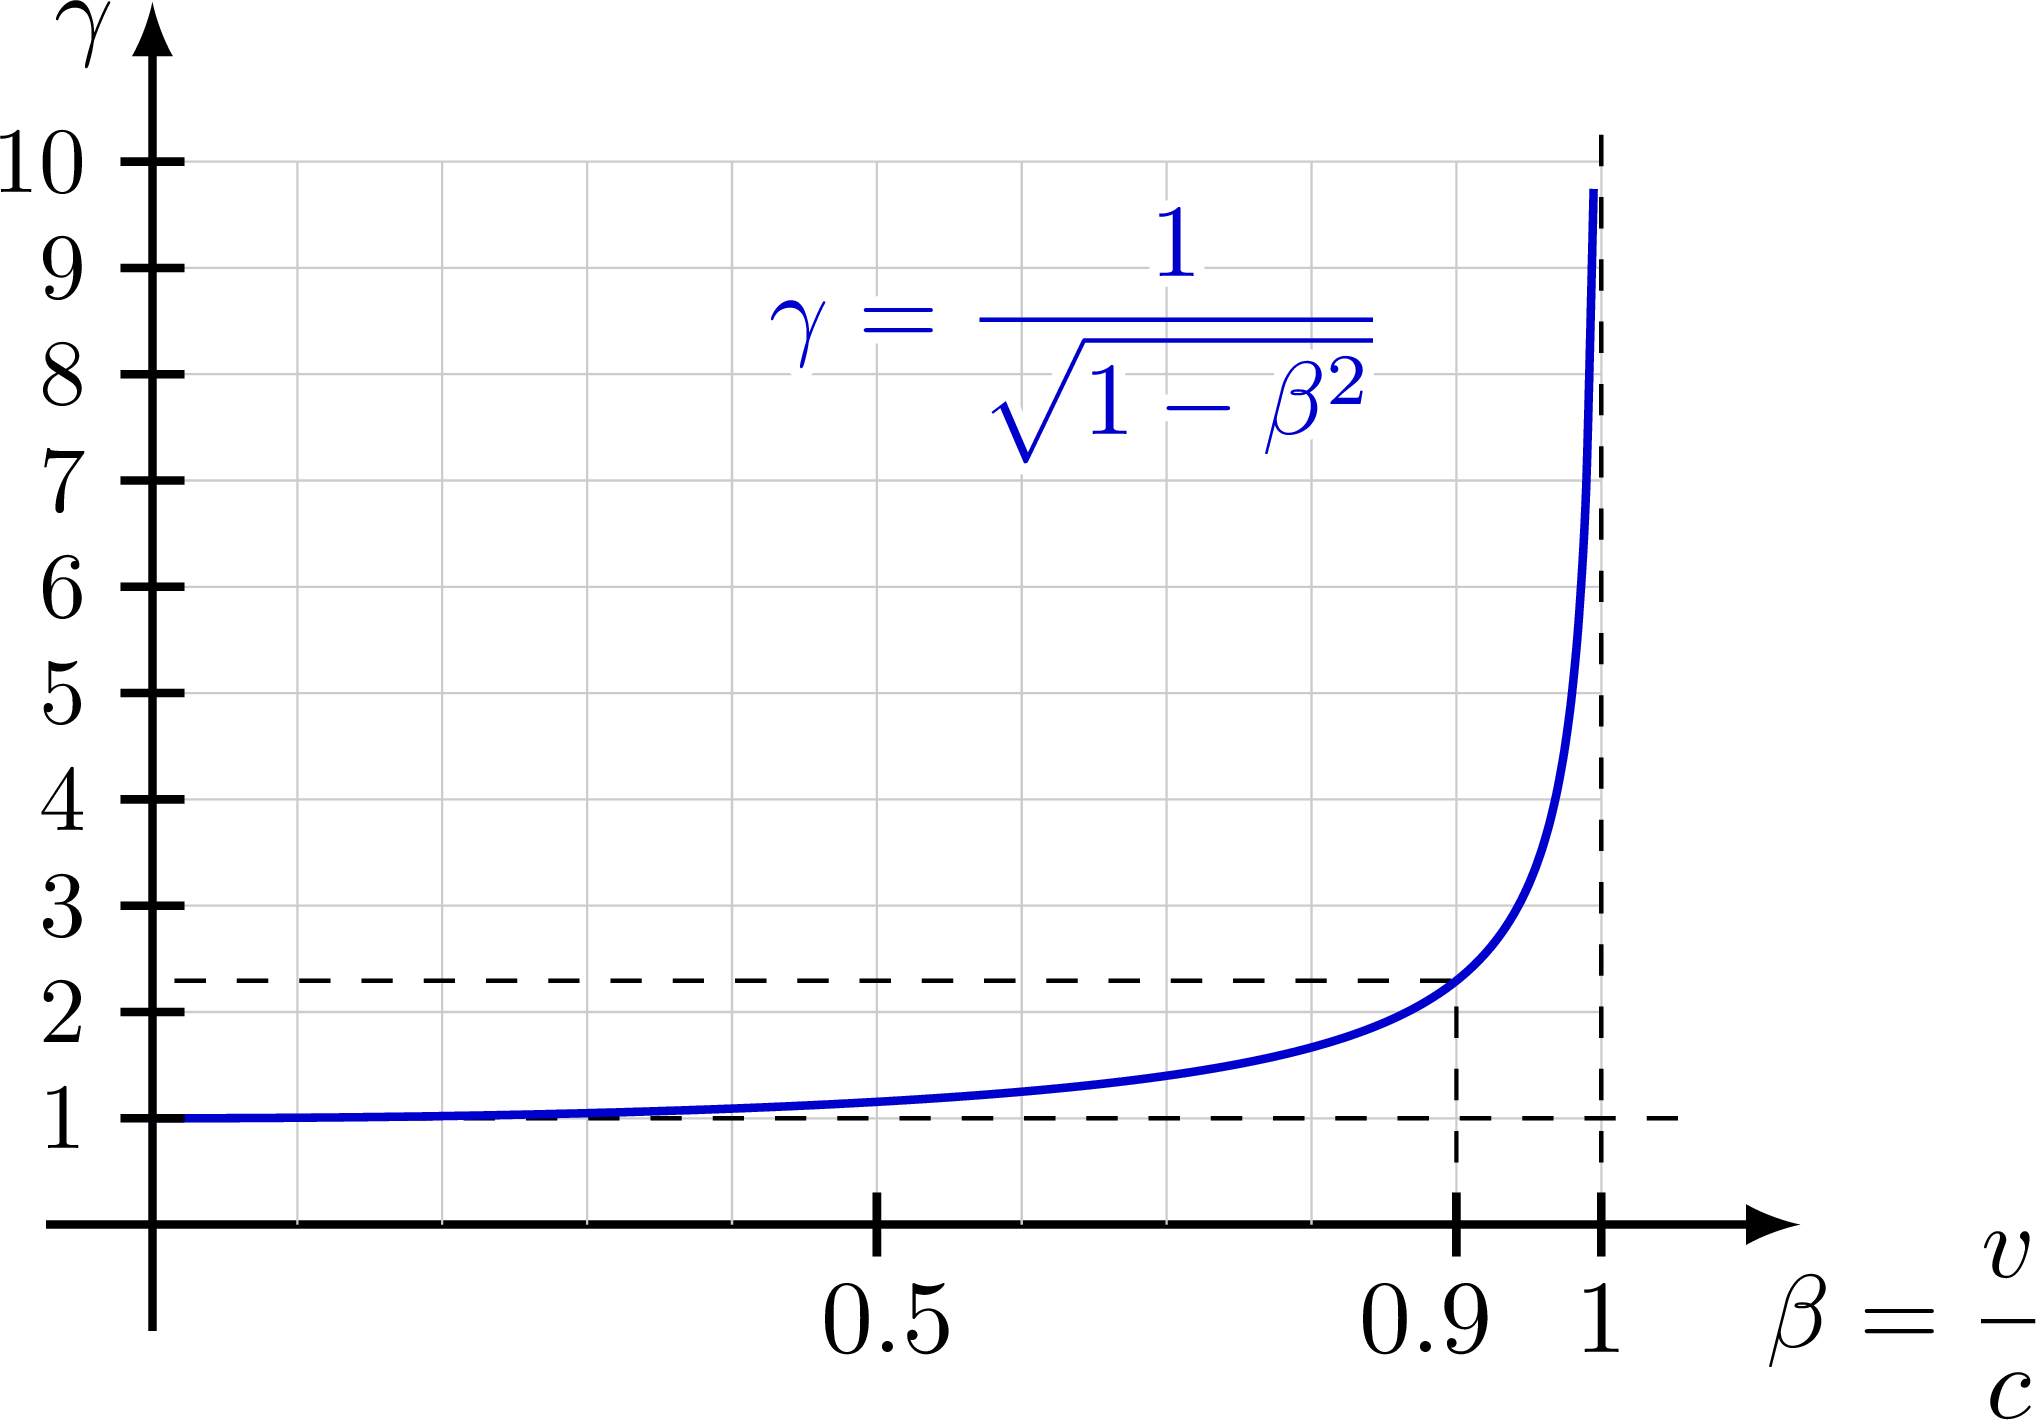
\includegraphics[width=0.5\linewidth]{img/gamma.png}
    \caption{The Lorentz factor $\gamma$ as a function of relative speed $\beta = v/c$. Note the rapid increase as $\beta$ approaches 1 \cite{tikz}.}
    \label{fig:gamma}
\end{figure}

% Hyperbolic rotations - Rindler coordinates

% \subsection{Relativistic effects}

\subsection{Length contraction}
A remarkable consequence of the Lorentz transformation is that observers in relative motion disagree on the length of objects measured parallel to the direction of motion. Consider a rod at rest in frame $S$, aligned along the x-axis, with endpoints at $x_A$ and $x_B$. Its length in its rest frame, the \textit{proper length}, is $L_0 = x_B - x_A$. To determine the length $L'$ of the rod as measured by an observer in $S'$ moving with velocity $v \mathbf{e}_x$ relative to $S$, the observer must measure the positions of the endpoints, $x_A'$ and $x_B'$, \textit{simultaneously} in their own frame, $S'$. This gives the length of the rod in $S'$ is $L' = x'_B - x'_A$. Let this simultaneous measurement occur at time $t'=0$ in $S'$.

From the inverse transformation for time in \eqref{coord-relations}, $t = \gamma(t' + \frac{vx'}{c^2})$. Setting $t'=0$, the times in frame $S$ corresponding to the measurements are $t_A = \gamma v x_A'$ and $t_B = \gamma v x_B'$. Note that these are generally different times in $S$. 

Now use the transformation for $x$ from \eqref{coord-relations} with simultaneous measurement in $S'$ implying $t'=0$ such that
\begin{align*}
    x_A &= \gamma \ x'_A, \\
    x_B &= \gamma \ x'_B.
\end{align*}
Therefore, the proper length of the rod in the rest frame is $L_0 = x_B - x_A = \gamma \ (x'_B - x'_A) = \gamma \ L'$. Rearranging this expression gives the length measured in the boosted frame $S'$ as
\begin{equation} \label{length-contraction}
    L' = \frac{L_0}{\gamma} = L_0 \sqrt{1-\beta^2}
\end{equation}
Since $\gamma \ge 1$, the length $L'$ is always less than or equal to the proper length $L_0$. This is the phenomena known as \textit{length contraction}. The contraction only occurs along the direction of motion while dimensions perpendicular to $\mathbf{v}$ remains unchanged according to \eqref{perp-transform}.

% \begin{align}
%     \label{time-component}
%     0 & = \gamma \left( t - \frac{vx}{c^2} \right) \implies t = \frac{vx}{c^2} \\
% \end{align}
% A remarkable consequence of the Lorentz transformation is that moving frames observe distances as shorter compared to stationary frames. Consider a rod placed along the x-axis in the rest frame $S$ in figure \ref{fig:two-frames} with its endpoints at $x_A$ and $x_B$. The length of the rod is given by $L_0 = x_B - x_A$. To determine the length of the rod $L'$ in $S'$, we must measure the end points at the same time $t'$ in $S'$, set arbitrarily to $t'=0$. Using \eqref{time-transform} we get
% Notice how the position of the endpoints measured simultaneously in $S'$ correspond to two distinct times $t_A$ and $t_B$ in $S$. Inserting these results into \eqref{space-transform}, we get the endpoints in $S'$ expressed in the unprimed coordinates
% \begin{align*}
%     x_A' &= \gamma\,(x_A - vt_A) = \gamma \, x_A \left( 1 - \beta^2 \right) \\
%     x_B' &= \gamma \, x_B \left( 1 - \beta^2 \right).
% \end{align*}
% The length of the rod in $S'$ is thus
% \begin{equation*}
%     L' = x_B' - x_A' = \gamma\,(x_B-x_A)(1-\beta^2).
% \end{equation*}
% With $L_0 = x_B-x_A$ and $\gamma=\frac{1}{\sqrt{1-\beta^2}}$, we arrive at a simple expression for $L'$ as
% \begin{equation}
%     L' = L_0\frac{1-\beta^2}{\sqrt{1-\beta^2}} = L_0\sqrt{1-\beta^2} = \frac{L_0}{\gamma}.
% \end{equation}

As visualized by figure \ref{fig:gamma}, when $v\to c,\ \beta \to 1 \implies \gamma \to \infty$, implying that the observed length $L'$ is considerably reduced at relativistic velocities and approaches zero as $v\to c$. For boosts in arbitrary directions, the directional dependence of \eqref{space-transform} indicates that length contraction along the parallel component leads to skewed geometry as suggested in figure \ref{fig:skewing}. This somewhat unintuitive effect is a characteristic feature of special relativity and is the primary phenomenon this project aims to visualize.

% This seemingly paradoxical result is a hallmark feature of special relativity. The
% This somewhat unintuitive effect is a characteristic feature of special relativity. It is straightforward to illustrate visually and highlights important aspects of the Lorentz transformation. As such, it is the main focus of this project.

\begin{figure}
    \centering
    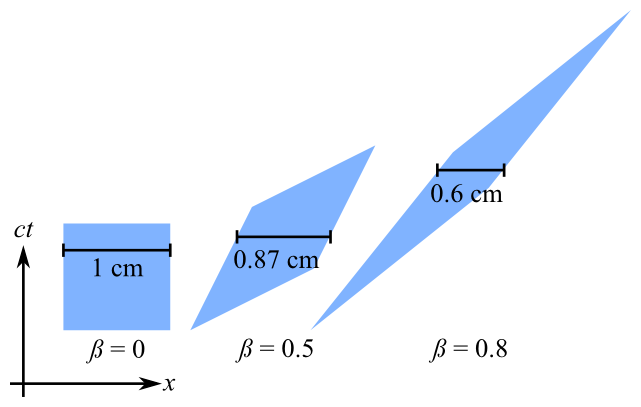
\includegraphics[width=0.5\linewidth]{img/skewing.png}
    \caption{Conceptual illustration of how length contraction, applied only along the direction of motion, can lead to skewing of objects viewed from a moving frame \cite{skew}.}
    \label{fig:skewing}
\end{figure}


% A direct consequence of the Lorentz transformation is \textit{length contraction}, wherein an object that is at rest in one inertial frame will appear shortened (contracted) along the direction of relative motion in another inertial frame moving at speed $v$. More concretely, if the object’s proper (rest) length is L, an observer in a frame where the object moves at speed $v$ will measure its length to be
% \begin{equation}
% L' = \frac{L}{\gamma} = L \sqrt{1 - \beta^{2}}.
% \label{eq:length_contraction}
% \end{equation}
% Notice that the only direction affected is the axis parallel to the motion; if the object is moving along the x-axis, then contraction occurs exclusively in the x-dimension. At everyday speeds, $\beta \sim 0,\ \gamma \approx 1 $ and the contraction is negligible. For velocities close to the speed of light, however, ∞ grows dramatically, causing a significant reduction in observed length.

% This effect can be difficult to visualize in standard terrestrial contexts because the velocities needed to produce an appreciable reduction in length are immense. By artificially lowering the speed of light in a simulation environment (or equivalently allowing a user-accessible velocity range that approaches the chosen $c$), we can bring the factor $\beta$ into an accessible regime where length contraction becomes visually apparent.

\subsection{Time dilation}
Another distinguishing relativistic phenomena is time dilation. Analogous to length contraction, observers in relative motion also disagree on the duration of time intervals. It is often summarized by the adage "moving clocks run slower".

Consider a clock at rest at a fixed position $x'$ in frame $S'$. It ticks at times $t'_A$ and $t'_B$, marking a time interval $\Delta t' = t'_B - t'_A$ in its own rest frame known as the \textit{proper time} of the clock. An observer in frame $S$, relative to whom the clock is moving with velocity $v \mathbf{e}_x$, measures these ticks occurring at times $t_A$ and $t_B$ in their frame.

Using the time transformation $t = \gamma(t' + \frac{vx'}{c^2})$ from \eqref{coord-relations}, we have:
\begin{align*}
    t_A &= \gamma(t'_A + vx') \\
    t_B &= \gamma(t'_B + vx')
\end{align*}
The time interval measured in frame $S$ is $\Delta t = t_B - t_A$. Subtracting the two equations gives
\begin{equation} \label{time-dilation}
    \Delta t = \gamma (t'_B - t'_A) = \gamma \Delta t'.
\end{equation}
Since $\gamma \ge 1$, the time interval $\Delta t$ measured in the frame where the clock is moving is always greater than or equal to the proper time interval $\Delta t'$ measured in the clock's rest frame. 

% While fundamental, visually simulating time dilation directly (e.g., slowing down animations or game logic based on relative motion) presents significant implementation challenges, especially within a standard game engine loop. Given the focus on geometric effects and the chosen CPU-based transformation approach, implementing robust time dilation was deemed outside the scope of this project.

 
% While the mathematical derivation is essentially similar to that of length contraction, it is considerably harder to intuit for students accustomed to fixed time. Moreover, 
While fundamental, simulating time dilation visually poses significant implementation challenges. Given the focus on geometric effects and the CPU-based transformation approach, implementing robust time dilation was deemed outside the scope of this project.
% it was deemed too computationally expensive and therefore excluded.

% Time dilation can be expressed by the adage "moving clocks run slower". Specifically, a time interval $\Delta t$ measured in a clock's rest frame appears dilated to $\Delta t'$ in a frame where the clock is moving, see figure \ref{fig:time-dilation}. The derivation follows a similar method as length contraction. Let $\Delta t = t_B - t_A$ in the rest frame of the clock. We have that
% \[
% t_A' = \gamma\left( t_A - \frac{v x_A}{c^2} \right),\quad 
% t_B' = \gamma\left( t_B - \frac{v x_B}{c^2} \right).
% \]
% The clock is stationary in the rest frame so $x_A = x_B$. $\Delta t'$ in the moving frame is then given by
% \begin{equation}
%     \Delta t' = t'_B - t'_A = \gamma \Delta t > \Delta t.
% \end{equation}

\begin{figure}
    \centering
    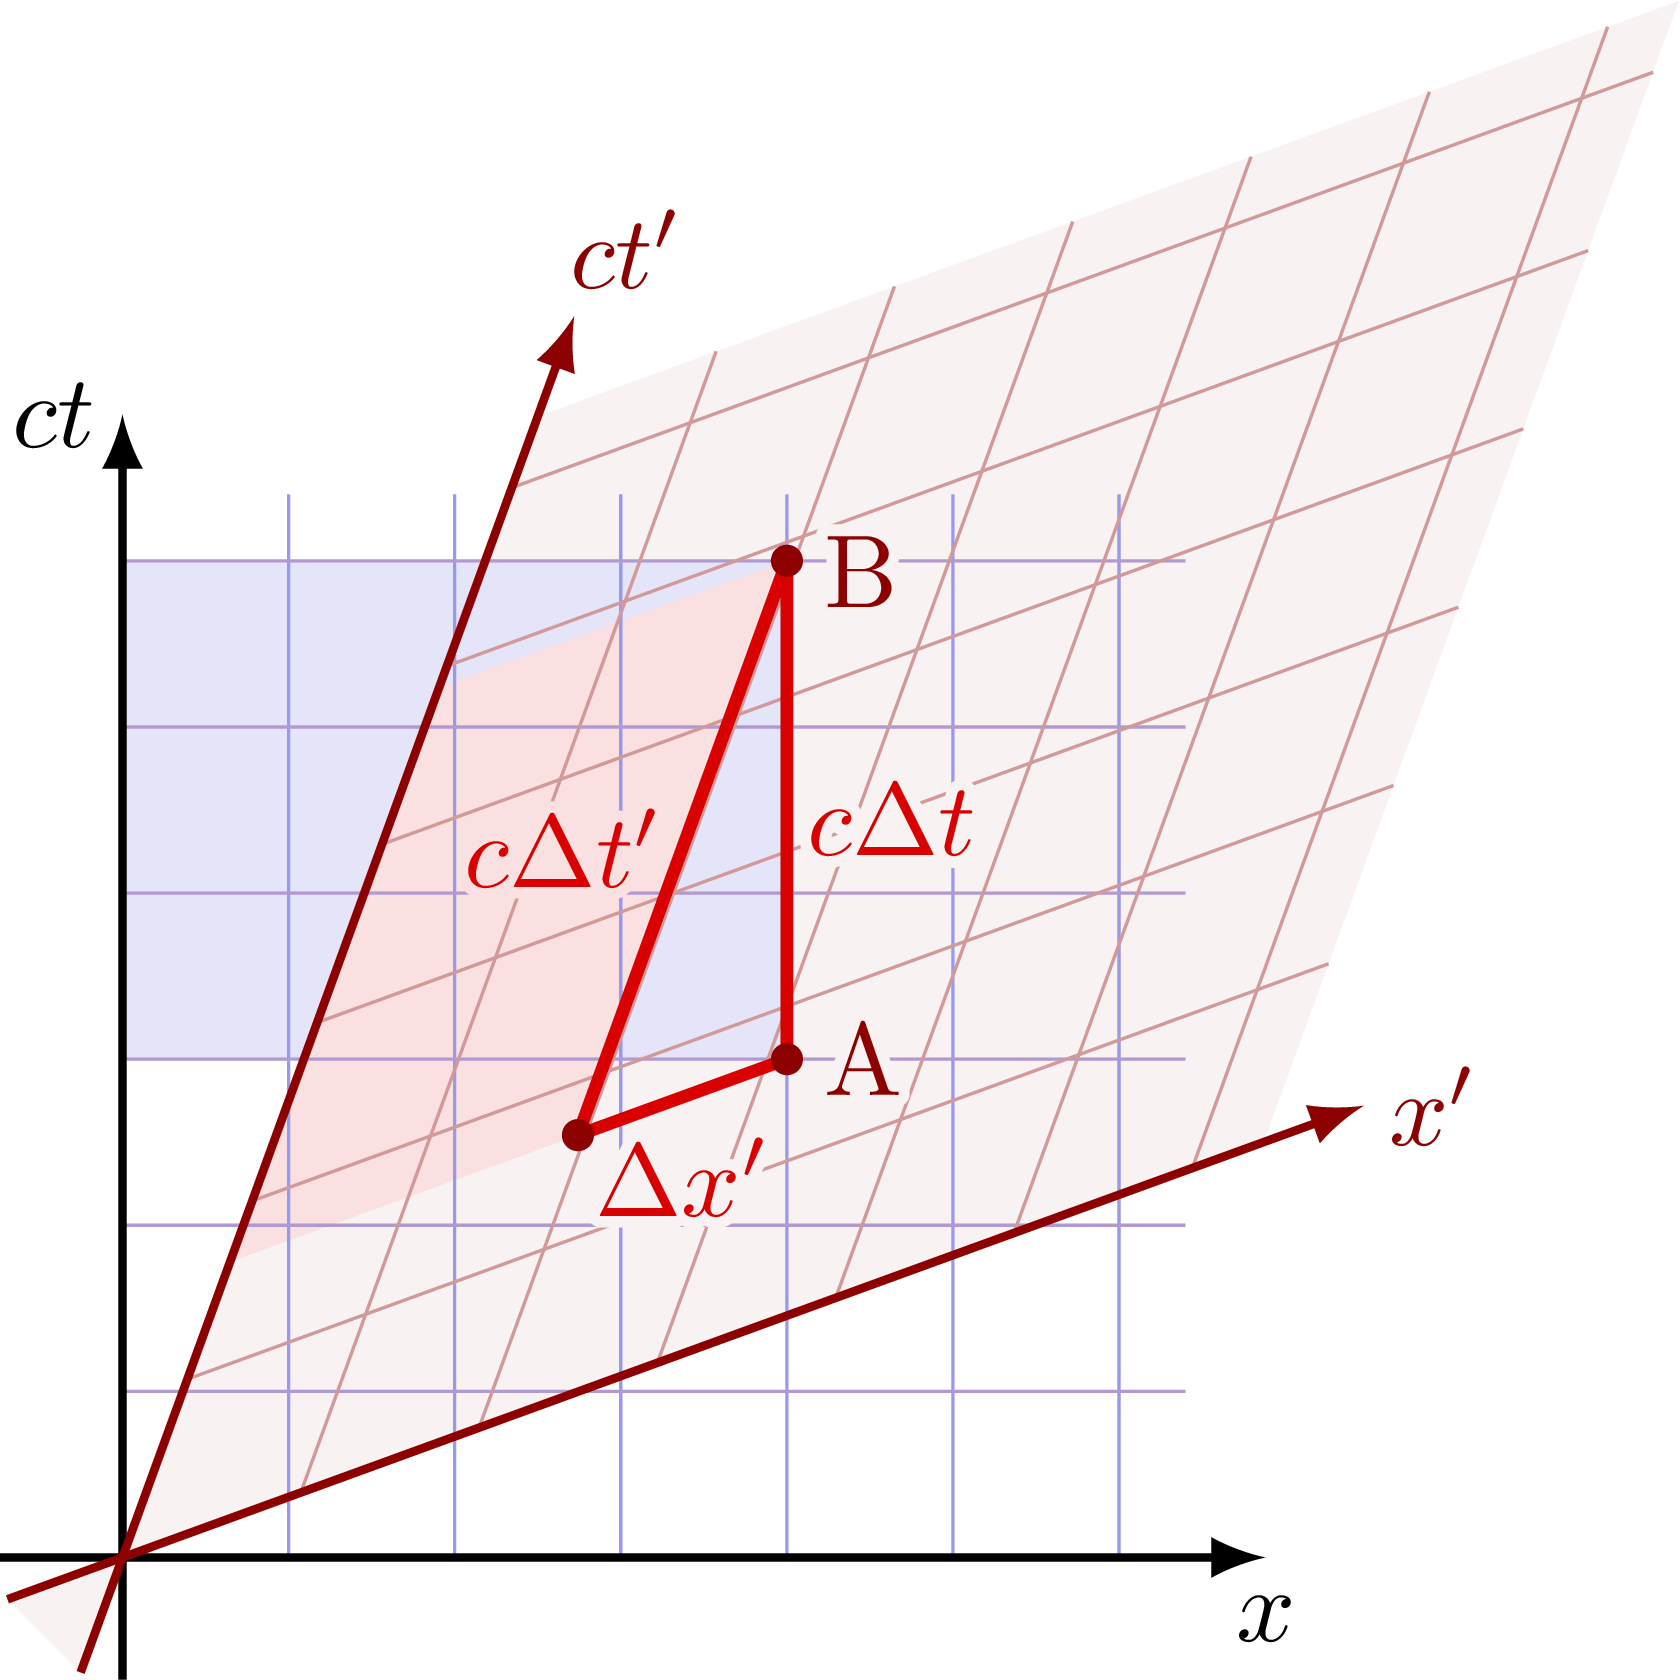
\includegraphics[width=0.49\linewidth]{img/time dilation 2.png}
    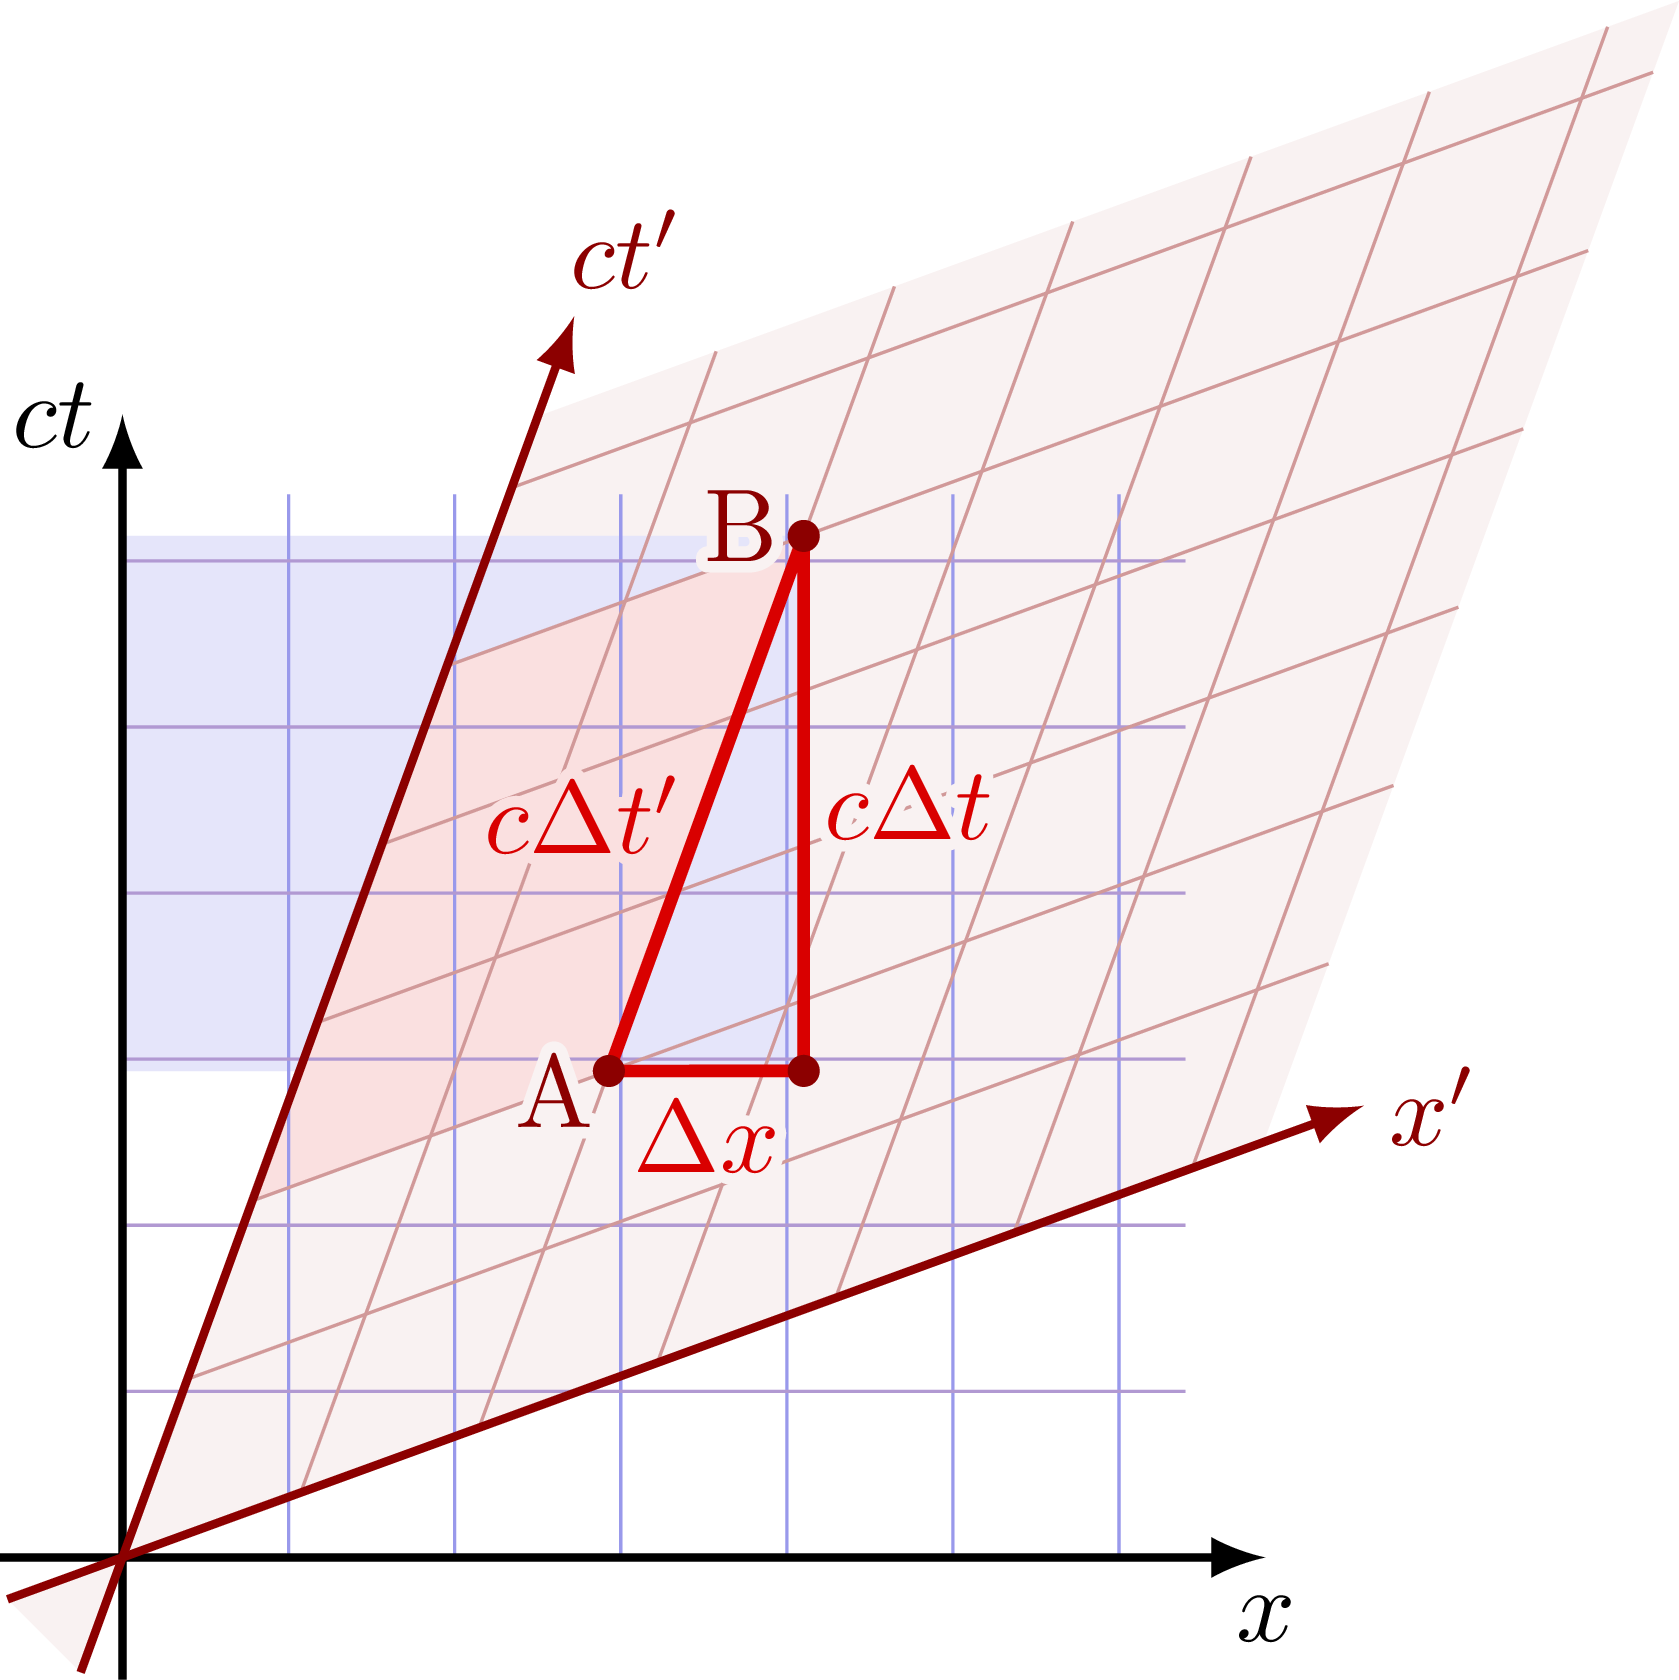
\includegraphics[width=0.49\linewidth]{img/time dilation 3.png}
    \caption{\textbf{Left:} Events A and B occur at the same location in the rest frame $S$ separated by the proper time $\Delta t$, signified by a vertical parallel to the $ct$ axis. In the boosted frame $S'$, A and B occur at different locations and are separated by a longer time interval $\Delta t' = \gamma \Delta t$.
    % Due to time dilation, A and B occur with a time separation of $\Delta t' = \gamma \Delta t > \Delta t$ in the boosted frame $S'$. 
    \textbf{Right:} A and B occur at the same location in the boosted frame $S'$. In $S$ the events occur at different locations separated by a longer time interval $\Delta t = \gamma \Delta t'$ \cite{tikz}.}
    \label{fig:time-dilation}
\end{figure}




% An additional manifestation of Lorentz invariance is \textit{time dilation}, meaning that a moving clock runs slower when observed from a frame in which it is in motion. Specifically, an elapsed time interval $\Delta t$ measured in a clock’s own rest frame appears dilated to $\Delta t'$ in a frame where the clock moves with speed $v$:
% \begin{equation}
%     \Delta t' = \gamma \Delta t
%     \quad\Longleftrightarrow\quad
%     \Delta t' > \Delta t.
% \end{equation}
% Like length contraction, this effect only becomes pronounced at large $\beta$. Both phenomena—length contraction and time dilation—stem from the underlying structure of Minkowski spacetime, in which different inertial observers slice up space and time in ways that preserve the interval $\Delta s^2$ but disagree on individual measurements of length and duration.


% --------------------- COMMENTS
% CMD + Shift + 7
% ---------------------

% Provide background to the problem area

% • Make it clear how the problem is relevant to
% physics and simulation

% • Cite relevant related literature and
% previous work from inside your text

% • Relevant math, equations

% • Show images – diagrams, related work
% images

% • This section does not need to be limited to
% the implementation that you did!

\subsection{Relativity of simultaneity}
The similarity between length contraction and time dilation stems from a fundamental principle that is critical to relativistic theory. As demonstrated in these effects, different frames with relative motion cannot agree that two spatially separated events happen at the same time. In other words, simultaneity is not absolute. This is known as the \textit{relativity of simultaneity} \cite{rindler}.

Consider the illustrations in figure \ref{fig:simultan}. The two events A and B are separated in space and time. In the rest frame $S$, A happens before B. However, in the boosted frame $S'$, B occurs before A.

\begin{figure}
    \centering
    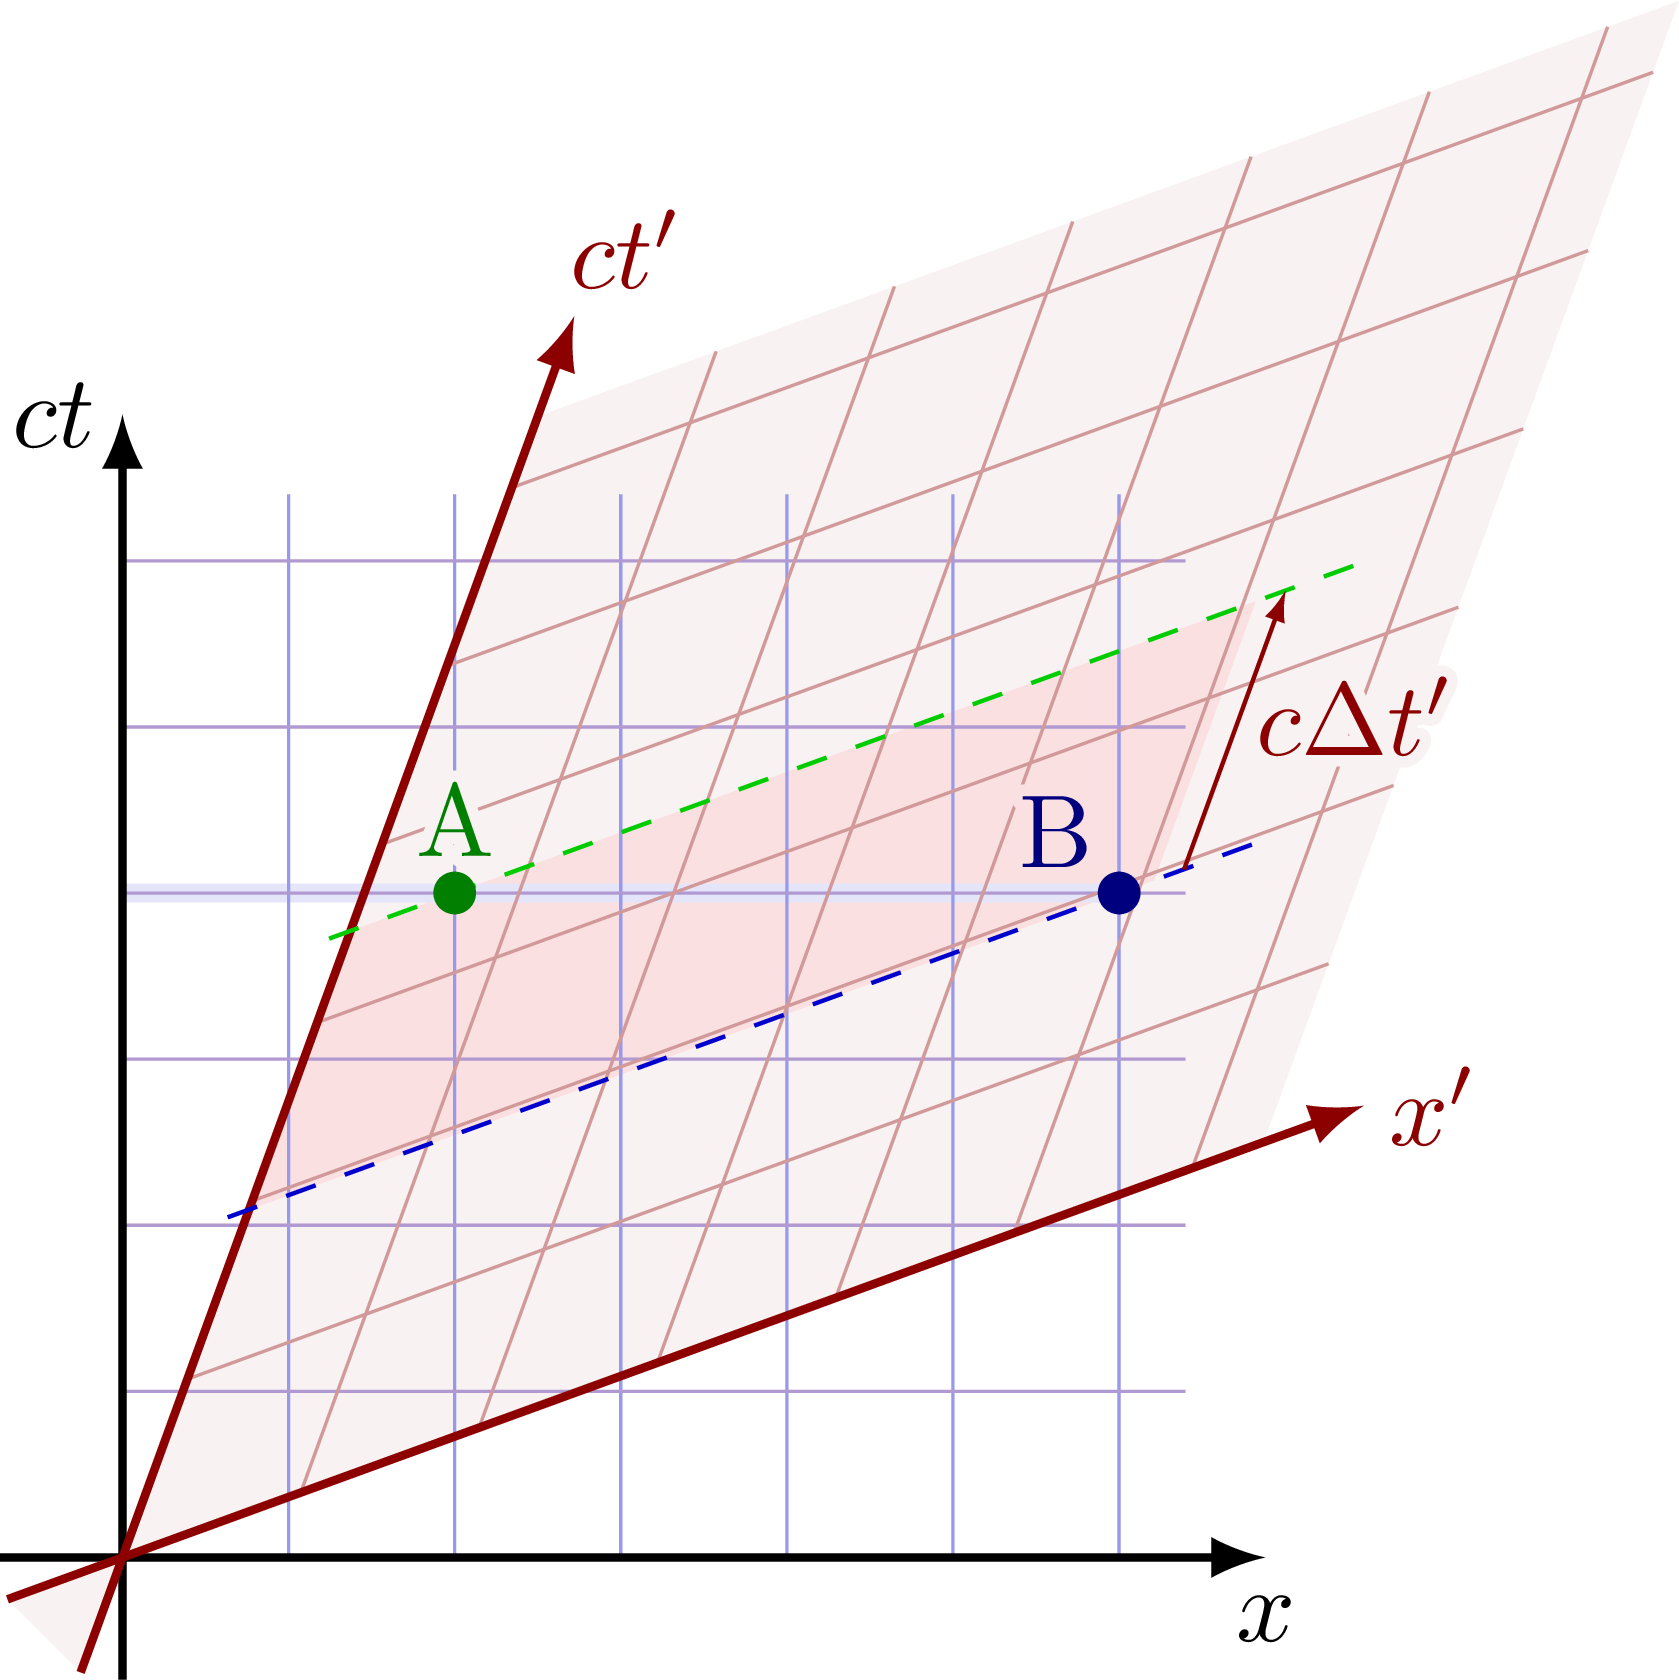
\includegraphics[width=0.33\linewidth]{img/simultaneity 1.png}
    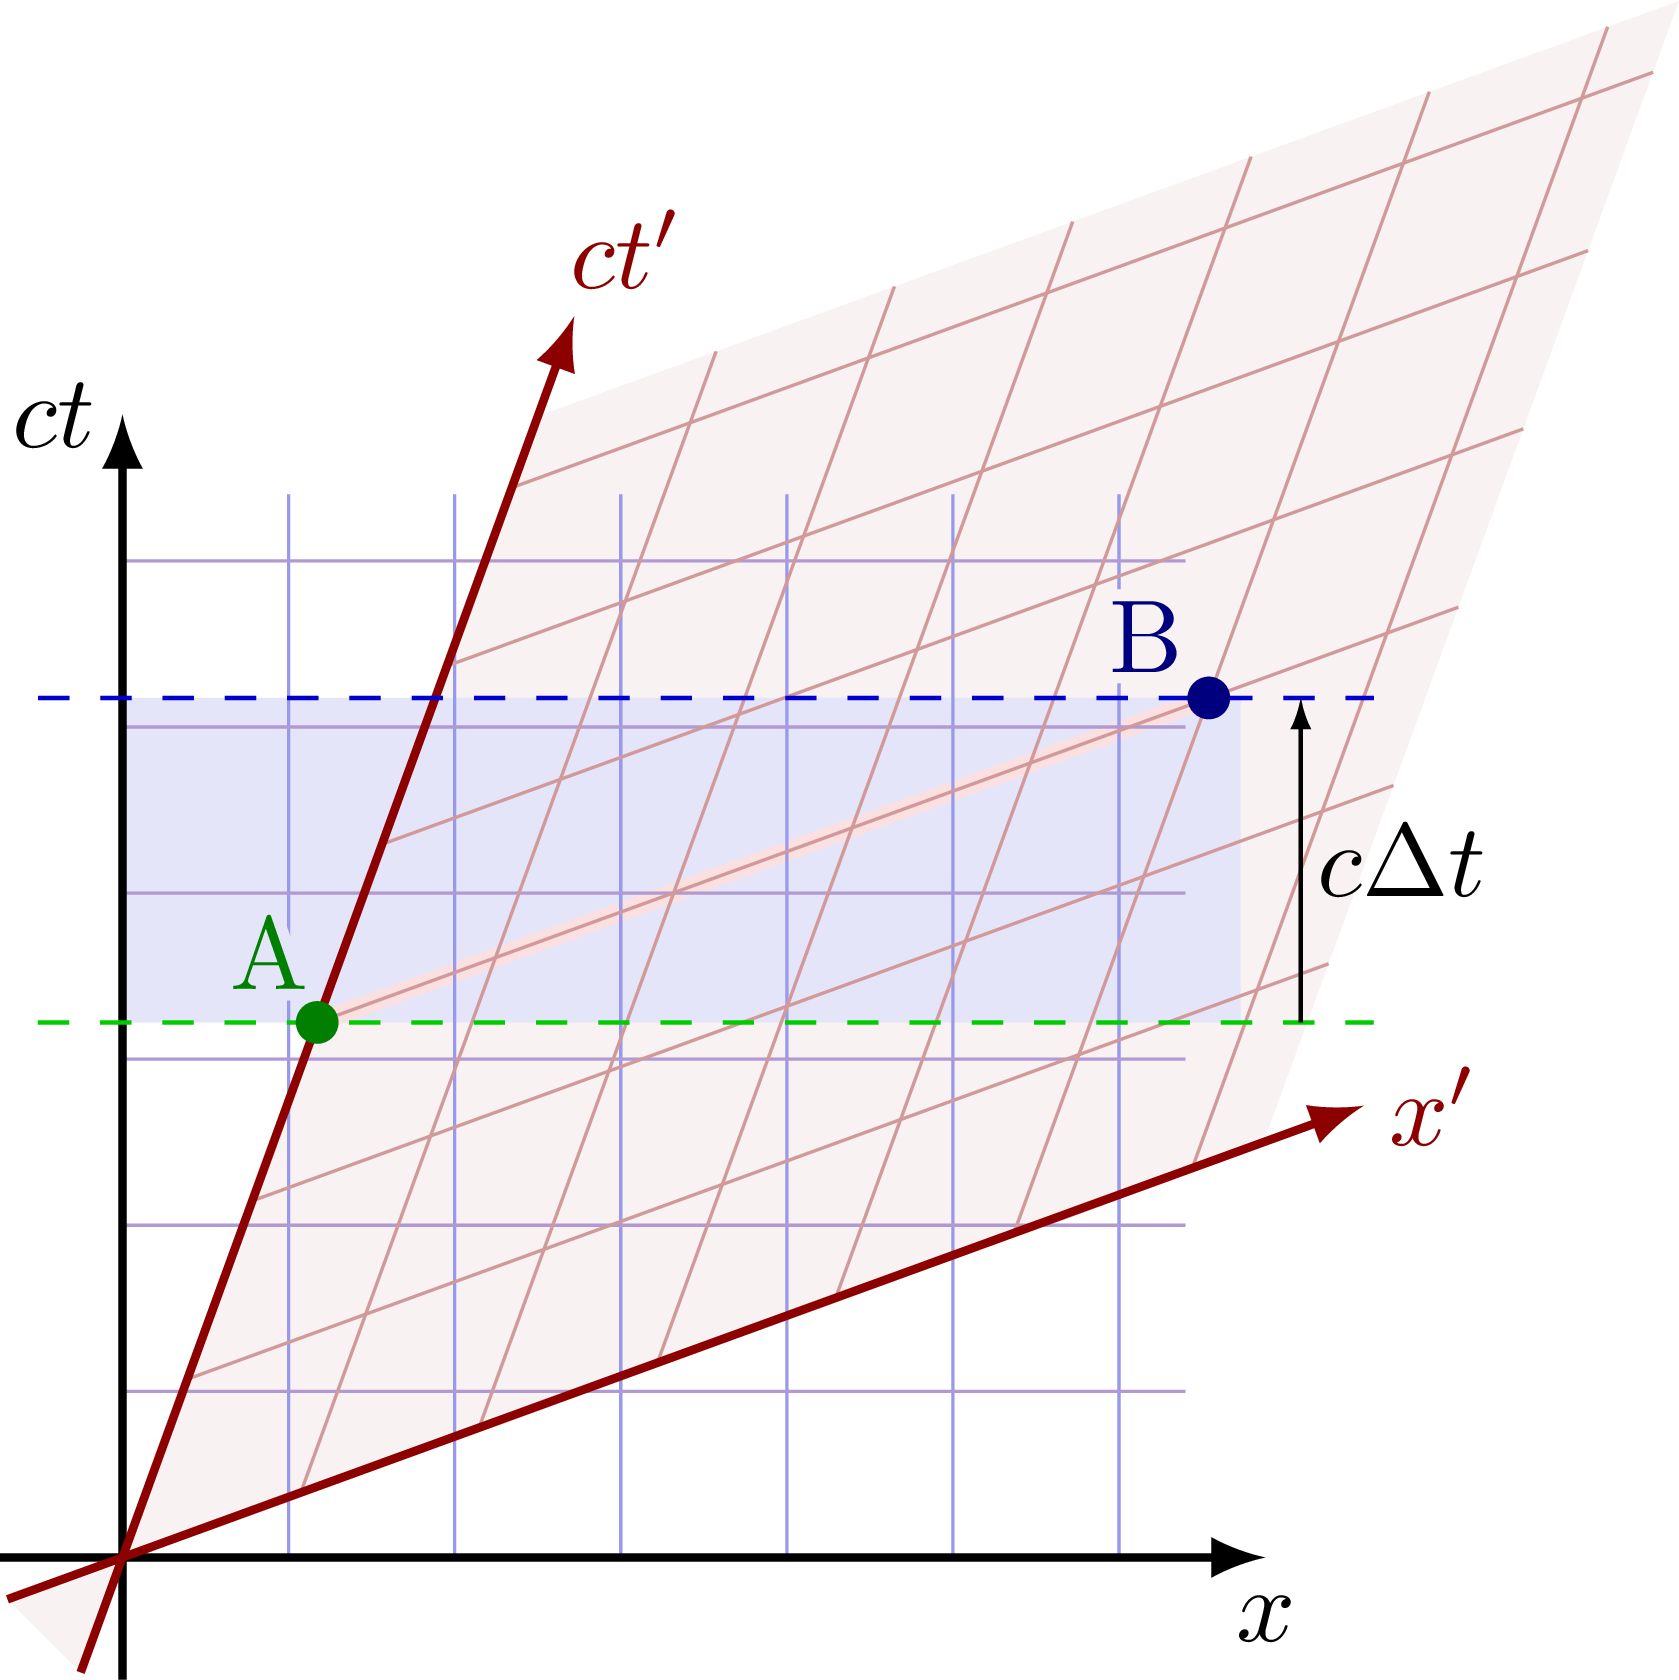
\includegraphics[width=0.33\linewidth]{img/simultaneity 2.png}
    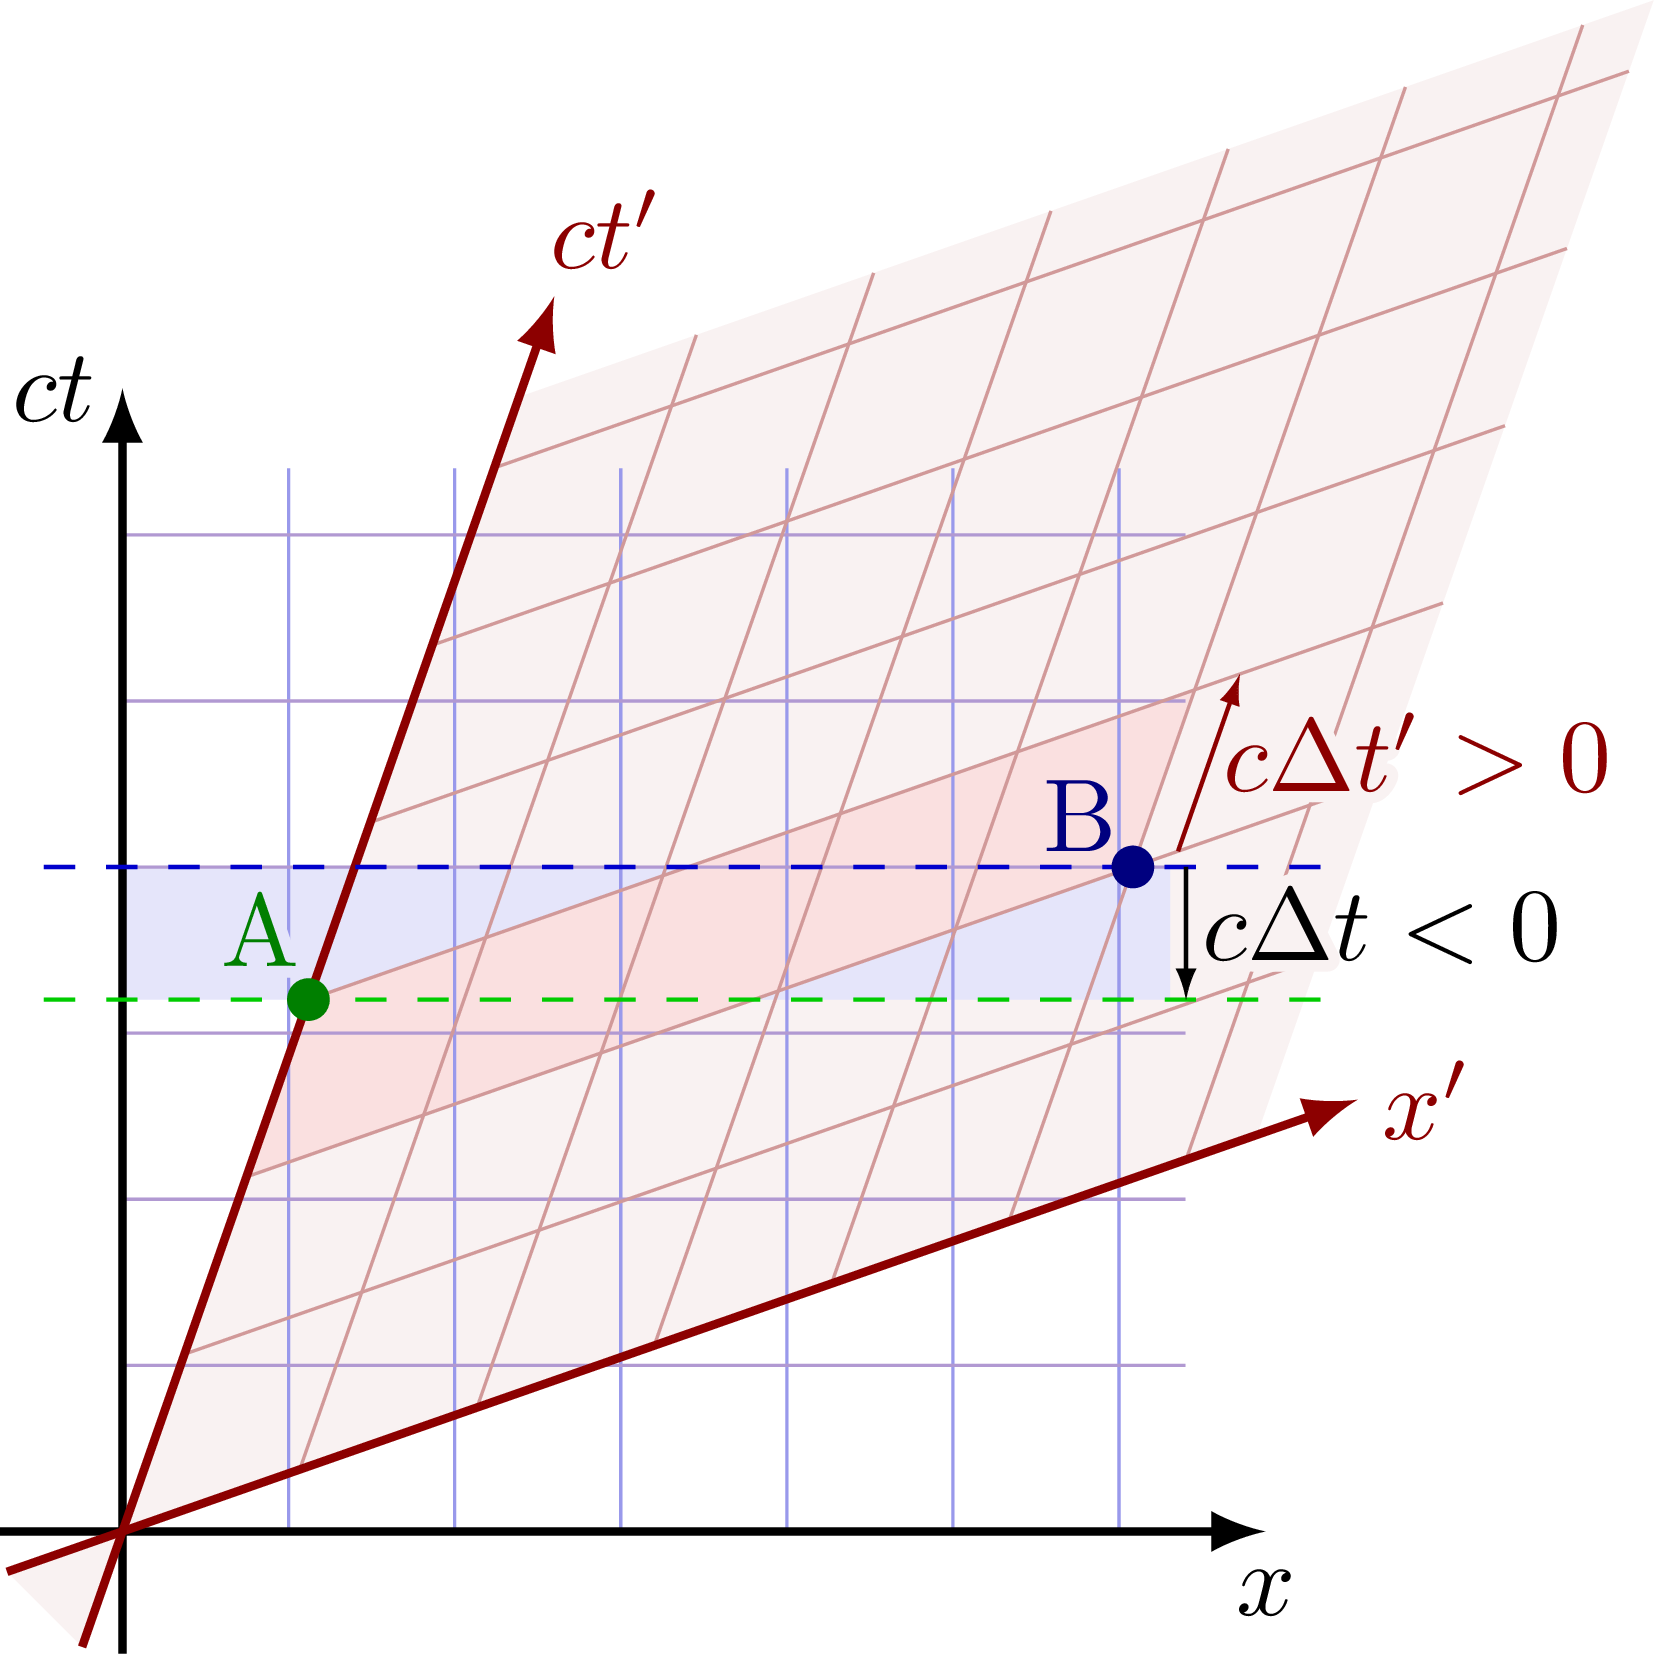
\includegraphics[width=0.33\linewidth]{img/simultaneity 3.png}
    \caption{ %\begin{multicols}{2}
    Visualization of the relativity of simultaneity. \textbf{Left:} two spatially separated events A and B are simultaneous in the rest frame. In the boosted frame, B happens before A. \textbf{Center:} A and B are simultaneous in the boosted frame but in the rest frame, A happens before B. \textbf{Right:} in the rest frame, A happens before B. In the boosted frame, B happens before A \cite{tikz}.
    % \end{multicols}
    }
    \label{fig:simultan}
\end{figure}


\subsection{Optical effects}
Relativistic motion does not only affect observed distance and time intervals, it also alters the visual appearance of moving objects. While this project focuses on the geometric effects on spacetime, a more realistic simulation needs to account for this, as demonstrated by OpenRelativity \cite{open-rel}, ReSim \cite{resim} and others.

At relativistic velocities, light waves will be subject to similar effects as subliminal waves of classical mechanics, such as Doppler shift and aberration of light. Light rays emitted from a stationary frame will appear to bend and change frequency, wavelength, amplitude angle when observed from a moving frame.

\paragraph{Relativistic aberration of light} occurs as an observer moves relative to a light source with relative velocity $v$. The angle of the incoming light rays $\theta'$ will be altered from the outgoing angle $\theta$, causing the observer to perceive the light rays as being emitted from a different direction. This is described by the formula
\begin{equation*}
    \cos\theta' = \frac{\cos \theta + \beta}{1+\beta\cos\theta} \Leftrightarrow
    \sin \theta' = \frac{\sin \theta}{\gamma(1+\beta \cos \theta)}.
\end{equation*}
When the observer moves towards the source, light rays will concentrate or "tunnel" in the forward direction, illustrated in figure \ref{fig:aberration}. This produces a curving effect of the field of view.
\begin{figure}[ht]
    \centering
    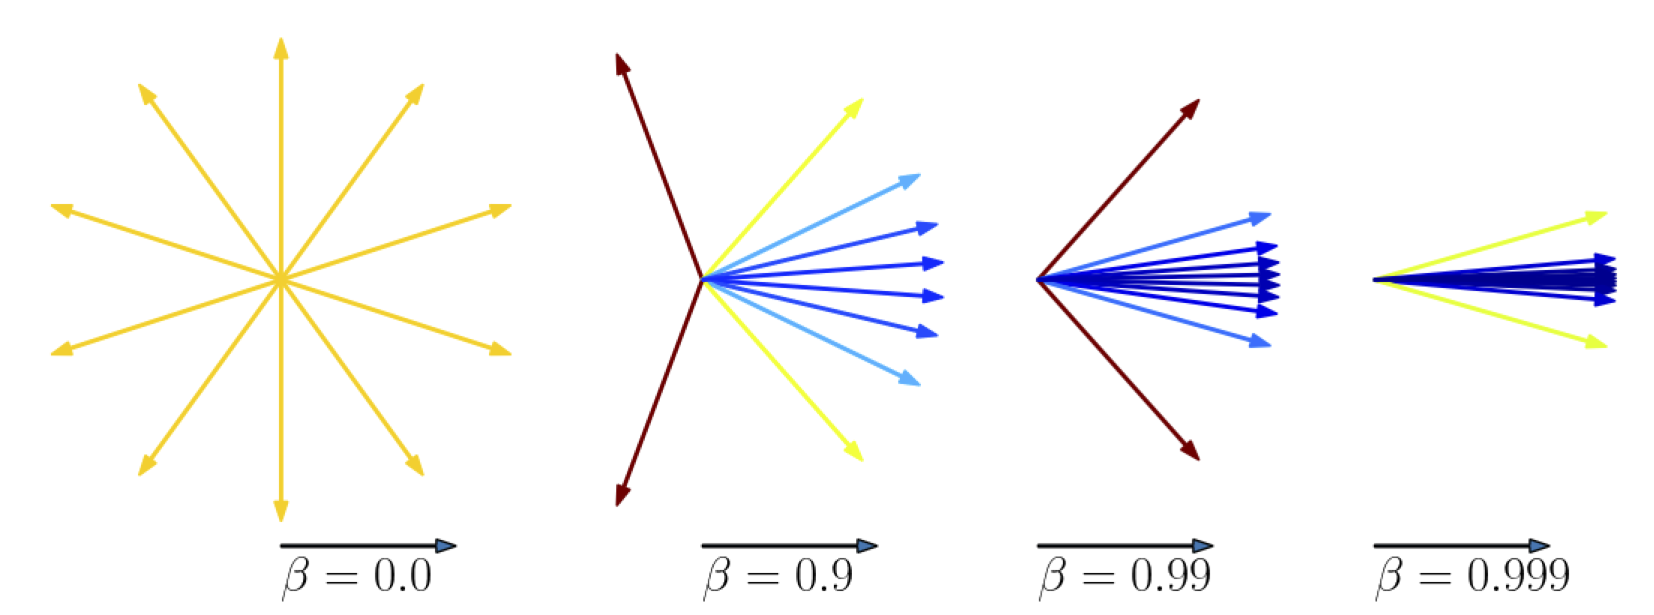
\includegraphics[width=0.8\linewidth]{img/aberration.png}
    \caption{Relativistic aberration of light \cite{aberration}.}
    \label{fig:aberration}
\end{figure}

\paragraph{Relativistic Doppler effect} is the relativistic generalization of the classical Doppler effect. The relative velocity between observer and source causes the emitted light ray to be received at a different frequency. When the relative motion is purely radial, the observed frequency $\nu$ is related to the emitted frequency $\nu_{0}$ as
\begin{equation}
    \frac{\nu_{0}}{\nu} = \sqrt{\frac{1+\beta}{1-\beta}}.
\end{equation}
The result of this frequency shift is that the light spectrum of approaching sources will appear blueshifted while receding sources will appear redshifted.


% This gives rise to optical effects such as bending and color shifts. 


% modeled as a plane wavefront

% how observers perceive spatial distances and time intervals; it also modifies the \emph{optical} appearance of moving objects. In other words, light rays themselves—how they are emitted, how they propagate, and how they are detected—are subject to transformations when there is relative motion near the speed of light. While this project primarily focuses on geometric effects like length contraction, a complete relativistic visualization system would eventually incorporate the following optical phenomena as well.

% \subsubsection{Relativistic aberration of light}
% \label{sec:relativistic-aberration}
% Relativistic aberration refers to the apparent change in the direction of incoming light due to high relative velocity between the source and the observer. In classical (Newtonian) physics, aberration can be understood as a change in the apparent angle because of the observer’s motion. However, at relativistic speeds, this effect is amplified by Lorentz transformations: the observed direction of a light ray is “pulled forward” (toward the observer’s velocity vector). As a result, objects that lie behind or to the side of an observer’s trajectory may still appear shifted toward the observer’s forward field of view when traveling at speeds close to \(c\).

% \subsubsection{Relativistic Doppler effect}
% \label{sec:relativistic-doppler}
% Another essential optical phenomenon is the \emph{relativistic Doppler effect}. It generalizes the classical Doppler shift to include both time dilation and aberration effects. Specifically, the frequency of light observed, \(\nu_{\text{obs}}\), relates to the emitted frequency, \(\nu_{\text{emit}}\), via
% \[
%     \nu_{\text{obs}} = \nu_{\text{emit}} \,\sqrt{\frac{1 + \beta}{1 - \beta}},
% \]
% for a purely radial motion with speed \(v=\beta c\). In more general three-dimensional configurations, one must account for the angle of emission and incorporate the aberration factor described above. 

\subsection{Implications for Real-Time Simulations}
Implementing these relativistic effects in a real-time simulation requires computationally expensive Lorentz transformations of each point in Minkowski spacetime for every frame. To address this, simulations must balance theoretical accuracy and performance constraints.

One technique utilized by many relativity simulation projects is to drastically reduce the speed of light, letting relativistic effects to manifest at speeds that humans are more accustomed to. While this approach is strictly unphysical, it provides a more intuitive context for the user while allowing the simulation environment to be constructed at a more manageable size.

One project that does this is the aptly named \textit{A Slower Speed of Light} \cite{slower}, a game developed by MIT Game Lab which later developed into the \textit{OpenRelativity} project \cite{open-rel}. The project is a toolkit for incorporating relativistic effects in Unity by using custom shaders to offload intensive calculations from the CPU. By placing heavier graphics operations on the GPU instead, OpenRelativity achieves realistic rendering without significantly sacrificing performance.

Other examples of similar projects relying on GPU shaders include Fons van der Plas' \textit{ReSim} \cite{resim}, which utilizes C\# and OpenGL, and the more recent \textit{special-relativity} by Harry Gifford \cite{harry} using WebGL. These methods demonstrate that GPU accelerated customs shaders make it possible to create realistic simulations of relativistic effects while retaining high performance. 

% Mathematically, one can derive relativistic aberration by examining how null vectors (\(\mathrm{d}s^2=0\)) in Minkowski spacetime transform under a velocity boost. In a simulation context such as Unity, implementing aberration often involves computing, for each rendered pixel or ray, the transformation of the incoming direction from the object’s emission frame to the observer’s frame. This can be done in a shader or via a custom raytracing algorithm. While more computationally demanding than geometric transformations alone, it provides a richer, more realistic depiction of how rapidly moving objects and backgrounds are visually distorted.

% From a simulation perspective, implementing a full Doppler shift requires either real-time spectral adjustments (e.g., shifting texture colors, adjusting emission wavelengths) or specialized rendering pipelines. In interactive scenarios, these shifts can be dramatic at high \(\beta\), illustrating how an approaching object becomes “blueshifted” and a receding object becomes “redshifted”.

% In a practical setting—such as a Unity-based simulation—carrying out transformations directly on coordinates (or vertices) allows one to illustrate length contraction dynamically as the relative speed $\beta$ changes. By selecting an artificial “speed of light” well within typical in-engine velocities, users can see how lengths in the forward direction contract visually, and how time intervals between events (e.g., frame updates, animations) can be stretched or compressed. These ideas form the theoretical grounding for the implementation detailed in the next sections.

% Such real-time demonstrations can greatly enhance conceptual understanding. Instead of passively reading about transformations, students can interactively perceive them: as they adjust velocity, objects in the simulated scene physically contract in the direction of motion, reinforcing the mathematical relationships derived above.

%-------------------------------------------------------------------
% ------------------------------------------------------------------
% Problem

\section{Problem} 
The physical manifestations of special relativity are rarely observed in everyday life, where velocities remain far below the speed of light. The mathematical framework of the theory is elegantly formulated but geometrically abstract. This project seeks to visualize the effects of Lorentz transformation between different frames of reference through an interactive 3D simulation built in Unity. By allowing users to control their velocity as they navigate an environment, the simulation aims to bridge the gap between theory and experience by visualizing relativistic effects to build intuitive understanding. Attain this goal required overcoming several conceptual and computational challenges.

\subsection{The speed of light}
A key obstacle of demonstrating relativistic physics is the immense speed of light: $c \approx 3 \times 10^{8} \ \text{m/s}$. At human-scale velocities, relativistic effects remain negligible. Creating a simulation at velocities closer to $c$ would require building and rendering a 3D environment at unfeasible scales.

The solution to this problem is inspired by a common notational trick. To simplify calculation, theoretical physicists often employ \textit{natural units} where the speed of light is normalized to 1. In the context of a simulation, this seemingly arbitrary notational convention functions as an artificial reduction of the speed of light. This is a common technique also employed by the other projects referenced above. Although unphysical, it enables length contraction to occur at ordinary velocities.





\subsection{Frames of reference}
% \begin{itemize}
%     \item The environment objects are assumed to be static, collectively defining a single inertial \textit{rest frame} ($S_{env}$).
%     \item The player moves with velocity $\mathbf{v}$ relative to this environment frame, defining the player's moving frame ($S_{player}$).
%     \item The simulation calculates how the static environment ($S_{env}$) appears when observed from the player's frame ($S_{player}$).
% \end{itemize}

From a simulation perspective, enforcing relativistic simultaneity across many moving objects is a complex undertaking. Since the simulation must account for and transform each point in spacetime in relation to the player, an independently moving environment would require the timing of events and updated positions to be calculated with respect to the moving observer at each frame.

To sidestep the full complexity of multi-frame simultaneity, the simulation in this project assumes a single rest frame for all objects in the environment. This is implemented in practice by requiring all environment objects to be static in their shared frame. The moving player, along with the camera, constitutes another, boosted frame. Calculations are then based on the relative velocity and position between environment and player. Since the user follows the player from a third-person perspective, they are observing from the rest frame of the player. As indicated by \eqref{inversetransform} and figure \ref{fig:boost}, it is equivalent to transform the player's boosted frame to the rest frame of the environment with velocity $\mathbf{v}$ and to transform the environment's boosted frame traveling at $-\mathbf{v}$ to the player's rest frame.



% To remedy this, a static environment reduces some of this complexity.

% - Static environment
% - Handling time in Unity



\subsection{Per-vertex transformation}
To get a proper Lorentz transformation of the scene, all points in the environment need to be 

This project takes another approach to vertex transformations that differs from the methods employed by previous projects outlined above. Instead of modifying Unity's render pipeline through custom shaders, all transformations are performed on the CPU. The reason behind this is that shaders are built in another programming language than C#. It was deemed too time consuming to learn a new environment. Furthermore, writing the simulation exclusively in C# facilitates the application of pen-and-paper methods to a 3D environment.

\subsection{Time-coordinate for the environment}


% \eqref{Lambda}

how unity handles spatial transformations (in rest frame of player)\\
how unity handles time (observed / proper time for player)\\
which objects to transform and how to get them\\
% illustration of lorentz boost

% how to perform

% what we want to do:
% \textbf{THE ENVIRONMENT}
% \begin{itemize}
%     \item perform lorentz transformation on all points in the environment.
%     \item the environment is static. $\frac{\text{d}x^\mu}{\text{d}t}=v^\mu=0$
%     \item In the rest frame of the environment,
%     \item all objects in the environment are children of one common parent.
%     \item objects therefore share the same origo
%     \item 
% \end{itemize}
% \textbf{THE PLAYER}
% \begin{itemize}
%     \item transform all points from the rest frame of the environment, $S$, to the rest frame of the moving player $S'$. 
%     \item In $S$, $S'$ appears Lorentz boosted with $v'^i = |\mathbf{v}_{\text{player}}|$
%     \item In $S'$, $S$ appears Lorentz boosted with $v'^i = -|\mathbf{v}_{\text{player}}|$
    
%     \item 
% \end{itemize}

% \ref{sec:implementation})

% \subsection{External resources}
\subsection{Generative tools}
Brief description of how generative AI was used in this project.
% Throughout the development of this project, I consulted ChatGPT as a supportive resource in several capacities. First, ChatGPT served as a research aid by helping me identify and compare similar open-source projects and reference materials relevant to relativistic simulations (such as MIT’s OpenRelativity). Second, it was useful for looking up documentation related to Unity’s handling of transforms, meshes, and vertex data—particularly when clarifying how per-vertex manipulation interacts with Unity’s rendering pipeline. 

% Beyond research, ChatGPT also provided coding tips and suggestions for debugging. For instance, when I encountered issues with floating-point inaccuracies or unexpected mesh distortions, ChatGPT offered alternative strategies (e.g., clamping small values or verifying transform hierarchies). Finally, ChatGPT contributed to the writing process itself by proofreading sections of text and suggesting improvements to ensure technical clarity and academic style. Importantly, the core design decisions—such as defining the specific per-vertex Lorentz transformation approach and integrating it into Unity’s update cycle—emerged from my own experimentation and research. ChatGPT’s role was therefore advisory and supportive, rather than a substitute for hands-on implementation.

% \section[]{Design \& Methodology}

% \subsection{Initial Project Specification}
% SEE APPENDIX A

% \begin{itemize}
%   \item Overarching goal: real-time transform of environment geometry under Lorentz transforms.
%   \item Mention single local player, partial usage of built-in Unity systems.
% \end{itemize}

% \subsection{Methodological Evolution}
% \paragraph{Older Approach: \texttt{WRelativisticSceneManager.cs}}
% \begin{itemize}
%   \item Summarize the anisotropic scaling method: original positions, partial scaling along velocity direction.
%   \item Limitations for angled surfaces or complex geometry.
% \end{itemize}

% \paragraph{New Approach: \texttt{VertexManager.cs}}
% \begin{itemize}
%   \item Per-vertex 4D transformation: store rest positions, apply Minkowski matrix each frame.
%   \item More comprehensive handling of arbitrary shapes.
% \end{itemize}

% \subsection{Engine \& Tools}
% \begin{itemize}
%   \item Unity, C\#, \texttt{Unity.Mathematics} usage.
%   \item Justify the environment choice (ease of scene management).
% \end{itemize}

% \subsection{Data Collection \& Testing}
% \begin{itemize}
%   \item Testing small rods or cubes for numeric accuracy vs.\ $\tfrac{1}{\gamma}$ results.
% \end{itemize}

% \subsection{Development Blog Integration}
% \begin{itemize}
%   \item Key updates from the blog: mention date-based decisions and discovered issues.
% \end{itemize}

% \subsection{Avoiding Shaders}
% \begin{itemize}
%   \item Rationale for not using GPU-based solutions: complexity, time constraints, debugging ease.
% \end{itemize}

% -------------------------------------------------------------
% Implementation


\section{Implementation}

\subsection{Implementation details: Per-vertex transformation and time coordinate}
This section now turns from theoretical underpinnings to the practical implementation visible in the project scripts. All cited code excerpts (e.g., from \texttt{VertexManager.cs} and \texttt{LorentzTransform.cs}) come from the Unity project environment, where we apply the Lorentz transformation to each vertex in real time.

\subsubsection{Handling the time component for each vertex}
% In the code, each vertex’s four-vector is constructed using an \emph{ad hoc} time-like component:
% \begin{verbatim}
% float t_env = Vector3.Dot(-betaVec, relativePos);
% float4 rest4 = new float4(t_env, relativePos.x, 
%                           relativePos.y, relativePos.z);
% float4 transformed = math.mul(L, rest4);
% \end{verbatim}
% Here:
% \begin{itemize}
%     \item \(\texttt{relativePos}\) is the spatial offset of the vertex from some reference point (the “scene origin” minus the player’s offset).
%     \item \(\texttt{betaVec}\) is the three-dimensional velocity vector scaled by \(\beta = v / c\).
%     \item \(\texttt{t\_env}\) is used as a notional time coordinate, proportional to the dot product of \(-\betaVec\) with the vertex position.
% \end{itemize}

\paragraph{Physical interpretation and limitations.}
% This choice effectively attempts to define a “slice” of simultaneity by assigning each vertex a time value that depends on its spatial position. In strict special relativity, simultaneity is relative, and for an object in standard configuration (length at rest in its own frame), we would often set all vertices to share the same \(\texttt{t\_env}\) in one chosen frame and then transform them into another frame. However, the project’s current approach includes:
% \begin{itemize}
%     \item \textbf{Dimension-mixing:} \(\texttt{t\_env} = \mathbf{-\beta}\cdot \mathbf{x}\) is dimensionally reminiscent of \((v/c)\times(\text{distance})\). If \(c=1\) in code units, this becomes something akin to “distance \(\times\) velocity.” Though numerically consistent for a simplified scenario, one must exercise caution about whether it aligns with a consistent Minkowski geometry for an entire extended object.
%     \item \textbf{Potential unphysical or partial coverage of relativity of simultaneity:} Because every vertex’s “time” is set by its position, the entire object may become skewed if it is large or if the transformation changes quickly. In a physically rigorous approach, one might define a global time for the object in its rest frame and transform all vertices from \((t=0, x_i, y_i, z_i)\) in that rest frame to \((t', x'_i, y'_i, z'_i)\) in the new frame. Instead, the current approach yields an approximate or partial representation that is, however, still sufficient for illustrating \emph{some} relativistic distortion.
% \end{itemize}

% In short, while this method \emph{does} produce a length-contraction-like effect, it is not a full simulation of the object’s worldvolume in spacetime. Rather, it is a computational device that allows dynamic, real-time transformations of geometry. For many educational visualization purposes, it successfully conveys the idea that high velocity leads to “shrinking” along the motion axis, even if the detailed concurrency assumptions differ from canonical textbook treatments.

\subsubsection{Performing the Lorentz transformation on vertices}
% Next, the code multiplies the 4-vector \(\bigl(t_{\mathrm{env}}, x, y, z\bigr)\) by a Lorentz matrix \(\mathbf{L}\). The matrix itself is assembled in \texttt{LorentzTransform.cs}:
% \begin{verbatim}
% float gamma = 1f / math.sqrt(1f - (beta * beta));
% float factor = (gamma - 1f) / (beta * beta);

% // Minkowski transform (column-major):
% lorentzMatrix = new float4x4(
%     new float4(gamma, g.x, g.y, g.z),
%     ...
% );
% \end{verbatim}
% Here, \(\beta\) is the speed ratio, and \(\gamma\) is the corresponding Lorentz factor. By multiplying the 4-vector \(\bigl(t, x, y, z\bigr)\) by that matrix, one obtains
% \[
%   \bigl(t',\,x',\,y',\,z'\bigr) \;=\;
%   \mathbf{L}\,\bigl(t, x, y, z\bigr).
% \]
% Because \(\mathbf{L}\) is a boost in the direction of \(\betaVec\), the resulting coordinates \(\bigl(x', y', z'\bigr)\) are \emph{contracted} along that axis.

% \paragraph{From transformation to apparent contraction (without the explicit \(\boldsymbol{L' = L/\gamma}\) formula).}
% To see how contraction naturally arises, consider a simple case of a line of vertices along the \(\hat{x}\) direction in the object’s rest frame:
% \[
%   \bigl(t=0,\; x_i,\; 0,\; 0\bigr).
% \]
% Applying a Lorentz boost along \(\hat{x}\), you get
% \[
%    \bigl(t'= -\gamma\,\beta\,x_i,\quad
%          x'=\gamma\,x_i,\quad
%          y'=0,\quad
%          z'=0\bigr).
% \]
% Even though we avoid the direct formula \(L' = L/\gamma\) in the code, the \(\gamma\)-dependent scaling of \(x_i\) means that if you measure the distance between two vertices along \(x\), you see a factor of \(\gamma\). In the user’s actual script, the transformation is performed in real time, so the player’s velocity can change, and each vertex’s position is updated accordingly, making the object appear to “shrink” more and more as the speed approaches the artificially lowered \(c\).  

% In the final step, \texttt{VertexManager.cs} converts each vertex’s \((x',y',z')\) back into world space and updates the mesh to reflect the new positions. The engine subsequently renders the object from the camera’s perspective, revealing the shape that is—by construction—contracted along the motion axis.

\paragraph{Educational context.}
% Even though the code’s time-component handling is a simplified approach, it delivers a \emph{qualitatively correct} contraction effect along the velocity direction. Students can see how an initially normal-sized object morphs into a flattened shape as \(\beta\) grows. The deeper principle behind this effect—\emph{Lorentz boosting each vertex in Minkowski spacetime}—underlies the entire script. Notably, because the code updates every frame, one can smoothly transition through different velocities and visually track the continuous deformation of 3D shapes, bridging the gap between abstract equations and tangible geometry.

\subsection{Player Movement \& Velocity Computation}
\begin{itemize}
  \item \texttt{PlayerController.cs} snippet for computing \(\beta\) and \(\gamma\):
  \[
    \beta = \frac{\|\mathbf{v}\|}{\text{MoveSpeed}}, 
    \quad
    \gamma = \frac{1}{\sqrt{1 - \beta^2}}.
  \]
  \item Show relevant code lines, highlight numerical stability concerns.
\end{itemize}

\subsection{Constructing the Lorentz Matrix}
\begin{itemize}
  \item \texttt{LorentzTransform.cs}: main loop building the $4\times4$ boost matrix.
  \item Fallback to identity if speed $<\!10^{-6}$ to avoid division by near-zero.
\end{itemize}

% \subsection{IMPORTANT!!! \\ How I handled time for static objects}

% \subsection{Anisotropic Scaling (Older)}
% \begin{itemize}
%   \item \texttt{WRelativisticSceneManager.cs}: parallel-projection approach, simpler but less general.
%   \item Results in partial illusions for objects exactly aligned with velocity.
% \end{itemize}

\subsection{Full Vertex Manipulation}
\texttt{VertexManager.cs}: storing \emph{rest} world vertices, applying Lorentz transformation matrix each frame.
% \begin{itemize}
%   \item \texttt{VertexManager.cs}: storing \emph{rest} world vertices, applying Lorentz transformation matrix each frame.
%   \item Steps:
%     \begin{enumerate}
%       \item Convert local vertex to world space (rest).
%       \item Build 4D vector $(t,x,y,z)$.
%       \item Multiply by $\Lambda$.
%       \item Re-map to object local space for drawing.
%     \end{enumerate}
%   \item CPU overhead trade-off for high fidelity.
% \end{itemize}

\subsection{Coordinate Offsets \& Time Calculation}
% \begin{itemize}
%   \item Explanation of partial attempts to incorporate $t_{\mathrm{env}}$.
%   \item Acknowledge a truly correct optical rendering also needs Doppler, etc.
% \end{itemize}

% \subsection{Implementation Notes \& Edge Cases}
% \begin{itemize}
%   \item Floating-point instabilities at high $\beta$.
%   \item Colliders or physics not fully updated in the final approach.
% \end{itemize}


% -------------------------------------------------------------
% Limitations
\subsection{Limitations \& Constraints}

Due to the limited time frame, the scope had to be narrowed considerably. A result of this was that there was not time to learn how to program shaders.

As a result, there was not adequate time to learn how to 


\section{Results}
\subsection{Visualization of Contraction}
\begin{itemize}
  \item Screenshots or references to the blog: rods, cubes, environment objects.
  \item Observed contraction along velocity axis matches $\tfrac{1}{\gamma}$ scaling.
\end{itemize}

% \subsection{Comparative Observations: Old vs.\ New}
% \begin{itemize}
%   \item The older approach was easy but inaccurate for angled objects.
%   \item The vertex-based transform is more robust physically, at higher CPU cost.
% \end{itemize}

\subsection{Consistency with Theory}
% \begin{itemize}
%   \item Demonstrate test rods, measure final length vs.\ $L/\gamma$.
%   \item Show small numeric differences due to float precision.
% \end{itemize}

\subsection{Performance and Limitations}
% \begin{itemize}
%   \item CPU overhead for large meshes.
%   \item No Doppler or real-time shading is currently done.
% \end{itemize}

\section{Discussion}

\subsection{Future development}
\begin{itemize}
    \item Time dilation
    \item Relativistic Doppler shift
    \item Relativistic aberration
    \item Rindler coordinates
\end{itemize}

\subsection{Reflecting on Development}
% \begin{itemize}
%   \item Learned the significance of rest-space data storage.
%   \item Real-time 4D transformations are feasible but require careful optimization.
% \end{itemize}


\vspace{2em}
\noindent

% \section[CODE]{Code}

% \subsection{style 1}

% \begin{algorithm}[H]
% \caption{VertexManager Initialization (Start)}
% \begin{algorithmic}[1]
% \IF{player is not assigned}
%     \STATE player $\leftarrow$ FindObjectOfType(\texttt{PlayerController})
% \ENDIF
% \IF{lorentz is not assigned}
%     \STATE lorentz $\leftarrow$ FindObjectOfType(\texttt{LorentzTransform})
% \ENDIF
% \IF{environmentRoot is not assigned}
%     \STATE environmentRoot $\leftarrow$ self transform
% \ENDIF
% \STATE sceneOrigin $\leftarrow$ environmentRoot.position
% \STATE meshFilters $\leftarrow$ environmentRoot.GetComponentsInChildren(\texttt{MeshFilter})
% \FOR{each mesh filter \texttt{mf} in meshFilters}
%     \STATE Create runtimeMesh as a copy of \texttt{mf.mesh}
%     \STATE Replace \texttt{mf.mesh} with runtimeMesh
%     \FOR{each vertex $v$ in runtimeMesh.vertices}
%         \STATE Compute world coordinate: $v_{world} \leftarrow$ mf.transform.TransformPoint($v$)
%     \ENDFOR
%     \STATE Store original world vertices in a MeshData structure
%     \STATE Add MeshData to meshObjects list
% \ENDFOR
% \end{algorithmic}
% \end{algorithm}

% \begin{algorithm}[H]
% \caption{VertexManager Update}
% \begin{algorithmic}[1]
% \STATE $L \leftarrow$ lorentz.GetLorentzMatrix()
% \STATE playerPos $\leftarrow$ player.transform.position
% \STATE $\betaVec \leftarrow$ player.BetaVec, $\gamma \leftarrow$ player.Gamma
% \STATE offset $\leftarrow$ playerPos $-$ sceneOrigin
% \FOR{each MeshData in meshObjects}
%     \FOR{each original vertex $v$ in MeshData}
%         \STATE relativePos $\leftarrow (v -$ sceneOrigin$) -$ offset
%         \STATE $t \leftarrow \langle -\betaVec,\, \text{relativePos}\rangle$
%         \STATE Form 4-vector: $(t,\, x,\, y,\, z)$ using relativePos
%         \STATE transformed $\leftarrow L \cdot (t,\, x,\, y,\, z)$
%         \STATE newRelative $\leftarrow (\,\text{transformed.y},\, \text{transformed.z},\, \text{transformed.w}\,)$
%         \STATE newWorldPos $\leftarrow$ playerPos $+$ newRelative
%         \STATE newLocal $\leftarrow$ InverseTransformPoint(newWorldPos)
%     \ENDFOR
%     \STATE Update MeshData.runtimeMesh.vertices with newLocal vertices
%     \STATE Recalculate mesh bounds
% \ENDFOR
% \end{algorithmic}
% \end{algorithm}

% \subsection{style 2}

% \noindent\textbf{VertexManager Main Loop:}
% \begin{enumerate}
%     \item \textbf{VertexManager Initialization:}
%     \begin{enumerate}
%         \item Check if \texttt{player} and \texttt{lorentz} are assigned; if not, search for them in the scene.
%         \item If \texttt{environmentRoot} is not set, use the current object's transform.
%         \item Set \texttt{sceneOrigin} to the position of \texttt{environmentRoot}.
%         \item Retrieve all child MeshFilter components under \texttt{environmentRoot}.
%         \item For each MeshFilter:
%         \begin{enumerate}
%             \item Create a runtime copy of the mesh to prevent altering the original asset.
%             \item Transform each vertex from local space to world space and store it.
%             \item Save this data in a MeshData object and add it to the meshObjects list.
%         \end{enumerate}
%     \end{enumerate}
    
%     \begin{enumerate}
%         \item Retrieve the player's velocity parameters: \texttt{Beta}, \texttt{BetaVec}, and compute \texttt{Gamma}.
%         \item If the speed (Beta) is very small, set the transformation matrix to identity to avoid precision issues.
%         \item Otherwise, calculate the factor $(\gamma - 1)/\beta^2$.
%         \item Construct the 4x4 Lorentz transformation matrix using the computed parameters.
%         \item Store the resulting matrix for use in transforming 4-vectors.
%     \end{enumerate}
    
%     \vspace{1em}
%     \item \textbf{Initialization (Awake/Start):}
%     \begin{enumerate}
%         \item Retrieve the Lorentz transformation matrix from the \texttt{lorentz} component.
%         \item Get the current player's position, velocity vector (for $\beta$), and compute $\gamma$.
%         \item Calculate an offset relative to \texttt{sceneOrigin}.
%         \item For each MeshData object:
%         \begin{enumerate}
%             \item For each original vertex:
%             \begin{enumerate}
%                 \item Compute its relative position from the scene origin minus the player's offset.
%                 \item Compute the time coordinate as the dot product of the negative $\beta$ vector and the relative position.
%                 \item Build a 4-vector (t, x, y, z) and apply the Lorentz transformation.
%                 \item Extract the spatial components, add the player's position to obtain the new world position.
%                 \item Convert the world position back into the mesh’s local space.
%             \end{enumerate}
%             \item Update the mesh with the new vertex positions and recalculate its bounds.
%         \end{enumerate}
%     \end{enumerate}
% \end{enumerate}

% \noindent\textbf{PlayerController Main Loop:}
% \begin{enumerate}
%     \item \textbf{Initialization (Awake/Start):}
%     \begin{itemize}
%         \item Retrieve CharacterController, PlayerInput, main camera, and locate the graphics child.
%         \item Initialize camera angles and store the initial position.
%     \end{itemize}
%     \item \textbf{Update Loop:}
%     \begin{enumerate}
%         \item Perform ground-check to determine if the player is on the ground.
%         \item Process user inputs to update movement direction and velocity.
%         \item Handle gravity and jumping mechanics.
%         \item Adjust camera rotation based on look input.
%         \item Move the character controller using the updated velocity.
%         \item Update a rolling animation by computing displacement of the player.
%     \end{enumerate}
%     \item \textbf{Supporting Routines:}
%     \begin{itemize}
%         \item \texttt{ProcessInput}: Computes desired direction and adjusts horizontal velocity.
%         \item \texttt{ProcessGravityAndJump}: Applies gravity or jump impulse based on grounded state.
%         \item \texttt{CameraRotation}: Clamps and applies camera rotation based on input.
%     \end{itemize}
%     \item \textbf{Relativistic Properties:}
%     \begin{itemize}
%         \item Compute \texttt{Beta} as the ratio of current speed to maximum speed (clamped to 0.99).
%         \item Compute \texttt{Gamma} using the Lorentz factor formula.
%         \item Calculate \texttt{BetaVec} as the normalized velocity scaled by \texttt{Beta}.
%     \end{itemize}
% \end{enumerate}

% \subsection{style 3}

% \begin{minted}[obeytabs=true,tabsize=4,baselinestretch=1,fontsize=\small]{csharp}
% function CsharpApplyGravityAndJump(player, jumpPressed)
% {
%     if player.isGrounded {
%         if jumpPressed {
%             player.velocity.y = sqrt(2 * player.jumpHeight * -player.gravity)
%         } else {
%             player.velocity.y = 0
%         }
%     } else {
%         player.velocity.y += player.gravity * Time.deltaTime
%     }
% }
% \end{minted}
% \begin{minted}[obeytabs=true,tabsize=4,baselinestretch=1,fontsize=\small]{c}
% function applyGravityAndJump(player, jumpPressed){}
%     if player.isGroundedther nothno
%         if jumpPressed
%             player.velocity.y = sqrt(2 * player.jumpHeight * -player.gravity)
%         else
%             player.velocity.y = 0
%     else
%         player.velocity.y += player.gravity * Time.deltaTime
% \end{minted}



% -------------------------------------------------------------
% Sources
{\titleformat{\section}
    {\large\bfseries\sffamily\color{navy}}
    {\thesection}
    {0em}
    {\MakeUppercase{#1}}
\addcontentsline{toc}{section}{References}
\printbibliography}

\begin{appendices}
\begin{subappendices}
% {\color{gray}\hrulefill}
\subsection{Source code}\label{appendix:code}

\subsection{Project specification}\label{appendix:specification}
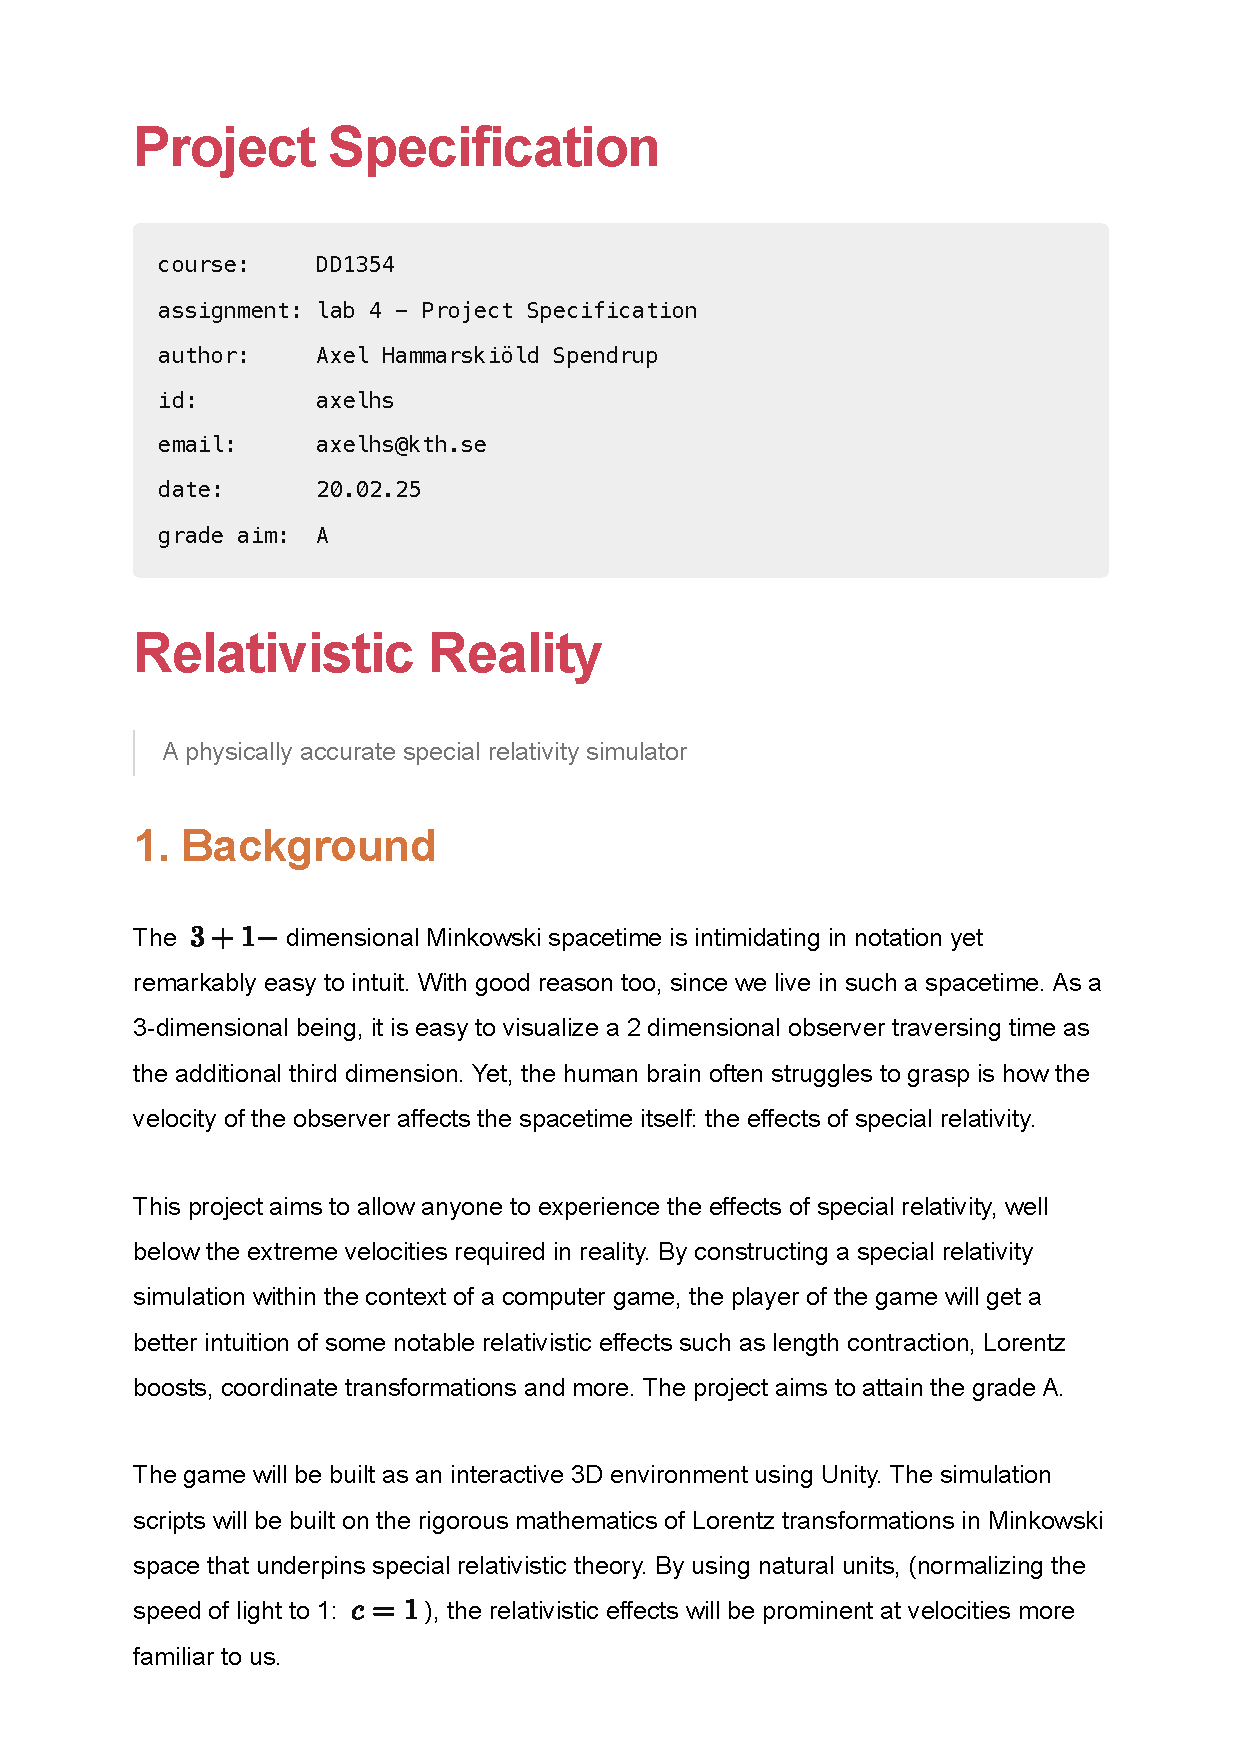
\includepdf[pages=-]{Project Specification.pdf}

\end{subappendices}
\end{appendices}




\end{document}
